\documentclass[10pt]{beamer}

\usetheme[progressbar=frametitle]{metropolis}
\usepackage{appendixnumberbeamer}

\usepackage{booktabs}
\usepackage[scale=2]{ccicons}

\usepackage{pgfplots}
\usepgfplotslibrary{dateplot}

\usepackage{braket} %ket vectors
\usepackage[font=footnotesize,labelfont=bf]{caption}
\usepackage{parskip} %automatic paragraphing
\usepackage{color}
\usepackage{cancel}
\usepackage{dsfont}%identity operator
\usepackage{mathrsfs}
\usepackage{xspace}
\usepackage{xcolor}
\usepackage{amsmath} %for gathering equations
\usepackage{amsfonts}
\usepackage{siunitx} %for SI units
\usepackage{pgfplots} %for plotting
%\usepackage{multimedia}
%\usepackage{media9}
\usepackage{xcolor,colortbl}
%\usepackage{fancyvrb}
%\usepackage{array}
\newcolumntype{C}[1]{>{\centering\let\newline\\\arraybackslash\hspace{0pt}}m{#1}}
\definecolor{darkyellow}{HTML}{FFB600}
\definecolor{emerald}{HTML}{32936F}
\definecolor{red1}{HTML}{FF0000}
\definecolor{red2}{HTML}{B20000}
\definecolor{red3}{HTML}{7F0000}
\definecolor{red4}{HTML}{FF3217}
\definecolor{red5}{HTML}{FF0D48}
\definecolor{blue1}{HTML}{0000FF}
\definecolor{blue2}{HTML}{0000B5}
\definecolor{blue3}{HTML}{000080}
\definecolor{blue4}{HTML}{3C00FF}
\definecolor{blue5}{HTML}{3C5DFF}
\definecolor{inputblue1}{HTML}{0000CC}
\definecolor{inputmixblue2}{HTML}{002DF7}
\definecolor{inputmixblue3}{HTML}{3C8BFF}
\definecolor{inputmixblue4}{HTML}{6730A8}
\definecolor{inputred1}{HTML}{970000}
\definecolor{inputmixred2}{HTML}{DF3100}
\definecolor{inputmixred3}{HTML}{C43335}
\definecolor{inputmixred4}{HTML}{DE366C}

\usepackage{filecontents} %for data loading
\begin{filecontents}{datax.dat}
0.06941, 28, 0.44096, 30, 0.15165, 25
0.04389, 146, 0.32707, 132,0.10722, 109
0.02823, 3622, 0.08416, 3478, 0.02086, 2997
0.01008, 17838, 0.005179, 17566, 0.01494, 14721
0.00165, 89130,0.0015799, 88216, 0.003327, 74009
0.00156, 444646, 0.0015601, 439060, 0.001578, 370813
%previous 3rd row: 0.04951, 728, 0.224107, 642, 0.020864, 601
\end{filecontents}
\begin{filecontents}{scatterplot.dat}
x y class
0.1 0.4 b
0.4 0.2 r
\end{filecontents}
\begin{filecontents}{scattered_example2.dat}
3.45, 643, 589, 3.76, 3.52
2.78, 558, 512, 2.87, 2.91
2.52, 583, 503, 2.54, 2.4
3.67, 685, 602, 3.83, 3.47
3.24, 592, 538, 3.29, 3.47
2.1, 562, 486, 2.64, 2.37 
\end{filecontents}

\usepackage[cal=zapfc,calscaled=.96]{mathalfa}

\newcommand{\themename}{\textbf{\textsc{metropolis}}\xspace}

\title{Quantum-enhanced machine learning: Implementing a quantum $k$-nearest\\ neighbour algorithm}
\subtitle{Bachelor thesis defense \newline 19. January 2017}
%\subtitle{19. January 2017}
%\date{\today}
\date{}
\author{Mark Fingerhuth\\ Supervisors: Dr. Fabrice Birembaut, Prof. Francesco Petruccione}
\institute{Maastricht Science Programme, Maastricht University, The Netherlands \newline Thesis work at the Centre for Quantum Technology,
University of KwaZulu-Natal\\ Durban, South Africa \newline
\begin{minipage}[c]{0.49\textwidth}
%\centering
%\textbf{Dr. Fabrice Birembaut}

\includegraphics[scale=0.3]{UM_logo.eps}
\end{minipage}%%%
%\hspace{0.5cm}
\begin{minipage}[c]{0.49\textwidth}
%\centering
%\hspace{1cm}\textbf{Prof. Francesco Petruccione}
\flushright
\includegraphics[scale=0.35]{logo.jpeg} 
\end{minipage}
}
% \titlegraphic{\hfill\includegraphics[height=1.5cm]{logo.pdf}}

\begin{document}

\maketitle

\begin{frame}{Table of contents}
  %\setbeamertemplate{section in toc}[sections numbered]
  %\tableofcontents %[hideallsubsections]
  \begin{enumerate}
  \item Introduction
  \item Machine Learning
  \item Quantum Computing
  \item Methods
  \item Quantum-enhanced Machine Learning
  \item Results: Amplitude-based quantum $k$-nearest neighbour algorithm
  \item Conclusion
  \item Outlook
  \end{enumerate}
\end{frame}


\section{Introduction}

{
\setbeamertemplate{frame footer}{\tiny{\textsuperscript{1}Bishop, C. M. (2006). Pattern recognition. Machine Learning, 128 .\newline \textsuperscript{2}Bekkerman, R., Bilenko, M., \& Langford, J. (2011). Scaling up machine learning: Parallel and distributed
approaches. Cambridge University Press.}}
\begin{frame}[fragile]{Enhancing machine learning with quantum mechanics}

\begin{minipage}[c]{0.45\textwidth}
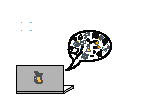
\includegraphics[scale=3.5]{Vectors/laptop_ml.eps}
\newline
\textbf{Machine learning}\\
Enable computers to\\
learn from data
\end{minipage}%%
\hspace{0.5cm}
\begin{minipage}[c]{0.49\textwidth}
%\flushright
\centering
%\includegraphics[scale=0.09]{google_car.jpeg}
\includegraphics[scale=0.8]{facial_recognition.jpg}\\
\vspace{-0.2cm}
\tiny{Source: IEEE Spectrum}
\normalsize
\vspace{0.5cm}
\flushleft
\begin{itemize}	 
%Approximately 2.5 quintillion (${10}^{18}$) bytes of digital data are created every day\textsuperscript{1}
	\item ML algorithms often involve\textsuperscript{1}
	\begin{itemize}
	\item solving large systems of linear equations
	\item inverting large matrices
	\item distance computations
	\end{itemize}
	\item Performing these computations on large data
sets gets increasingly difficult\textsuperscript{2}
\end{itemize}
\end{minipage}


\end{frame}
}

{
\setbeamertemplate{frame footer}{\tiny{\textsuperscript{1}}}
\begin{frame}[fragile]{Enhancing machine learning with quantum mechanics}
\hspace{-0.7cm}
\begin{minipage}[c]{0.59\textwidth}
\centering
\includegraphics[scale=0.16]{ibm-quantum-computer.jpg}\\
%\includegraphics[scale=0.12]{dwave.jpg}\\
\tiny{Sources: IBM}
\vspace{0.1cm}
\flushleft
\normalsize
\begin{itemize}
\item Quantum mechanics is about vectors in complex Hilbert spaces
\item Quantum computers are performing linear operations on qubits
\item Many-qubit systems are described by large vectors that can be manipulated in parallel on quantum computers
\item Machine learning involves manipulation of large vectors and matrices
\end{itemize}
\end{minipage}%%
\hspace{0.3cm}
\begin{minipage}[c]{0.39\textwidth}
\vspace{2.8cm}
\centering
\hspace{-1cm}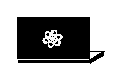
\includegraphics[scale=2.2]{Vectors/laptop_q.eps}
\flushleft
\textbf{Quantum computing}\\
Build computer hardware based on quantum physics
\end{minipage}

\end{frame}
}

{
\setbeamertemplate{frame footer}{\tiny{\textsuperscript{1}}}
\begin{frame}[fragile]{Enhancing machine learning with quantum mechanics}

\begin{figure}
\centering
%\hspace{2cm}
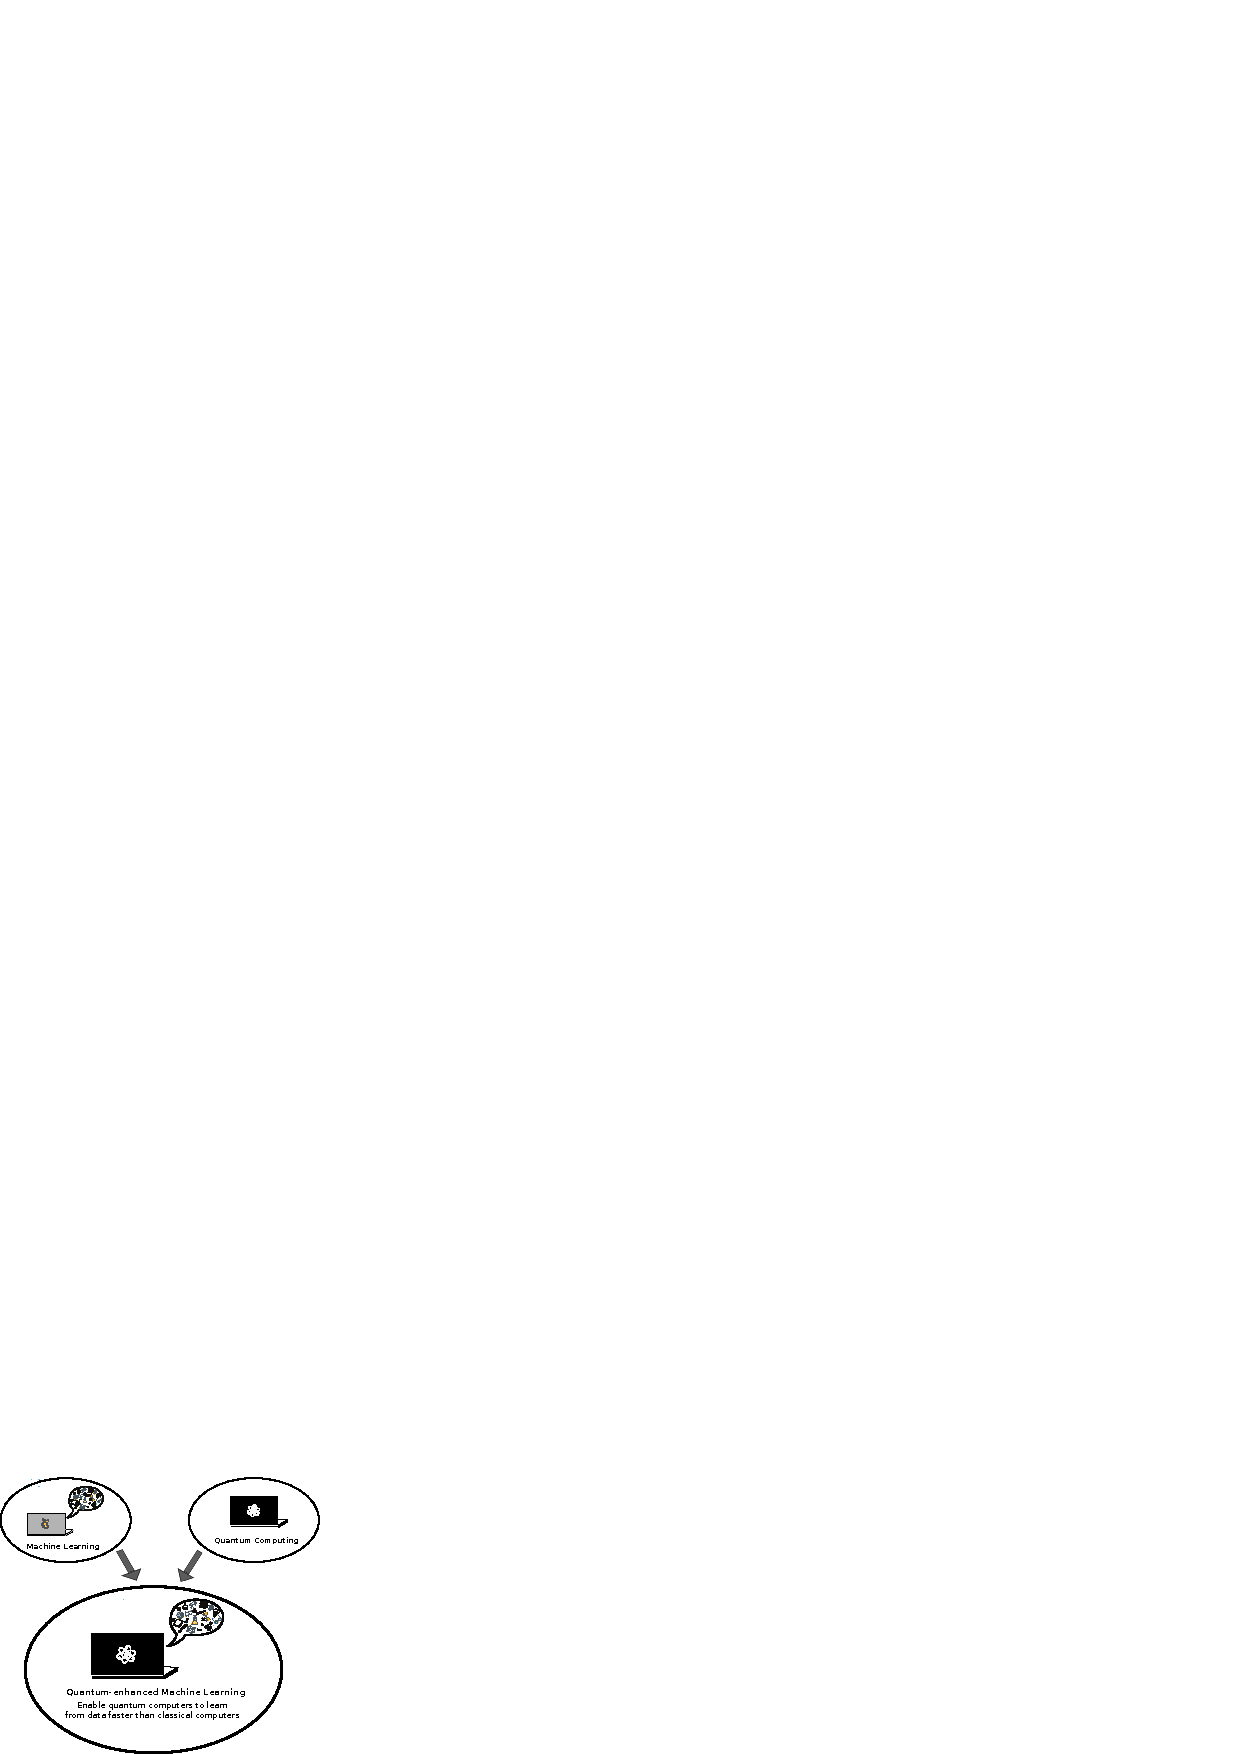
\includegraphics[scale=1.7]{Vectors/laptop_qml_flowchart.pdf}
\end{figure}
%\centering
%\textbf{Quantum-enhanced machine learning}\\
%Enable quantum computers to learn from data\\
%faster than classical computers

\end{frame}
}


\section{\protect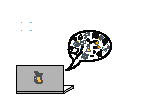
\includegraphics[scale=3.5]{Vectors/laptop_ml.eps}\newline Machine Learning
}

{
\setbeamertemplate{frame footer}{\tiny{\textsuperscript{1}}}
\begin{frame}[fragile]{Supervised machine learning}

\metroset{block=fill}

\begin{exampleblock}{The problem statement}
Given a dataset of inputs and their corresponding outputs,\\ predict the output of a new unknown input.
\end{exampleblock}

%\begin{equation}
%f(x) = o\, .
%\end{equation}

\vspace{1cm}
\begin{table}
\begin{tabular}{l  l }
\toprule
Input & Output\\\midrule
faces & emotions\\
heartbeat & healthy or sick\\
last year's daily weather & tomorrow's weather\\
message of a users & intention of text content\\
search history of a user & chance of clicking on a particular ad\\
\end{tabular}
\end{table}

%\begin{itemize}
%\item Labelled training dataset $\rightarrow$ supervision!
%\end{itemize}

%\begin{table}
%\begin{tabular}{| C{0.45cm} | C{1cm} |C{1.4cm} |}
%    \toprule
%      ID & Colour & Class label\\
%      \midrule
%       1 & \cellcolor{red1} & red \\\midrule
%       2 &\cellcolor{red2} & red \\\midrule
%       3 & \cellcolor{red3} & red \\\midrule\midrule
%       4 & \cellcolor{blue1} & blue \\\midrule
%       5 & \cellcolor{blue2} & blue \\\midrule
%       6 & \cellcolor{blue3} & blue \\
%      \bottomrule
%    \end{tabular}
%    \caption{Example training dataset.}
%\end{table}

%\begin{equation}
%f(x) = o\, .
%\end{equation}
%\begin{equation}
%f(\colorbox{red2}{colour}) = red\, .
%\end{equation}
%\begin{itemize}
%\item Labelled training dataset $\rightarrow$ supervision!
%\end{itemize}

\end{frame}
}

{
\setbeamertemplate{frame footer}{\tiny{\textsuperscript{1}}}
\begin{frame}[fragile]{Classical $k$-nearest neighbour with distance-weighting}

\centering{
%- kNN is a non-parametric classifier\\
- $k$ is a positive integer%, usually chosen small
}

\begin{minipage}[t]{.32\textwidth}
Given training dataset:\\
${D}_{T}$ = ${v}_{0}, {v}_{1},..,{v}_{16}$ \\
$v_{i} \in$ \{$red$, $blue$\}
\end{minipage}
\hspace{0.1cm}
\vline
\hspace{0.1cm}
\begin{minipage}[t]{.53\textwidth}
\flushright
Given a new vector $\tilde{x}$ (black halfcircle):\\
- consider $k$ nearest neighbours\\
- classify $\tilde{x}$, based on majority vote,\\as \emph{red} or \emph{blue}
\end{minipage}

\begin{minipage}[c]{0.49\textwidth}
\centering
$k = all$
\vspace{0.1cm}
\flushleft
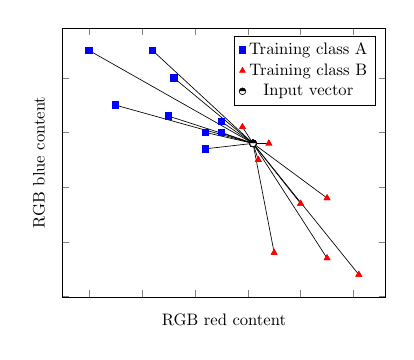
\begin{tikzpicture}[scale=0.6]
\begin{axis}[legend pos=north east,
ylabel={RGB blue content},
      xlabel={RGB red content},
 yticklabels={,,},
      xticklabels={,,},
			scatter/classes={
			a={mark=square*,blue}, 												b={mark=triangle*,red}, 											c={mark=halfcircle*,draw=black}}]
			\addplot[scatter,only marks, scatter src=explicit symbolic]
table[meta=label] {
x y label
0.15 -0.15 a
0.25 -0.17 a
0.26 -0.1 a
0.22 -0.05 a
0.35 -0.18 a
0.32 -0.2 a
0.32 -0.23 a
0.35 -0.2 a
0.42 -0.25 b
0.44 -0.22 b
0.39 -0.19 b
0.45 -0.42 b
0.55 -0.32 b
0.61 -0.46 b
0.5 -0.33 b
0.55 -0.43 b
0.41 -0.22 c
};
\addplot[scatter, scatter src=explicit symbolic]
table[meta=label] {
x y label
0.15 -0.15 a
0.41 -0.22 c
};
\addplot[scatter, scatter src=explicit symbolic]
table[meta=label] {
x y label
0.25 -0.17 a
0.41 -0.22 c
};
\addplot[scatter, scatter src=explicit symbolic]
table[meta=label] {
x y label
0.26 -0.1 a
0.41 -0.22 c
};
\addplot[scatter, scatter src=explicit symbolic]
table[meta=label] {
x y label
0.22 -0.05 a
0.41 -0.22 c
};
\addplot[scatter, scatter src=explicit symbolic]
table[meta=label] {
x y label
0.35 -0.18 a
0.41 -0.22 c
};
\addplot[scatter, scatter src=explicit symbolic]
table[meta=label] {
x y label
0.32 -0.2 a
0.41 -0.22 c
};
\addplot[scatter, scatter src=explicit symbolic]
table[meta=label] {
x y label
0.32 -0.23 a
0.41 -0.22 c
};
\addplot[scatter, scatter src=explicit symbolic]
table[meta=label] {
x y label
0.35 -0.2 a
0.41 -0.22 c
};
\addplot[scatter, scatter src=explicit symbolic]
table[meta=label] {
x y label
0.42 -0.25 b
0.41 -0.22 c
};
\addplot[scatter, scatter src=explicit symbolic]
table[meta=label] {
x y label
0.44 -0.22 b
0.41 -0.22 c
};
\addplot[scatter, scatter src=explicit symbolic]
table[meta=label] {
x y label
0.39 -0.19 b
0.41 -0.22 c
};
\addplot[scatter, scatter src=explicit symbolic]
table[meta=label] {
x y label
0.45 -0.42 b
0.41 -0.22 c
};
\addplot[scatter, scatter src=explicit symbolic]
table[meta=label] {
x y label
0.55 -0.32 b
0.41 -0.22 c
};
\addplot[scatter, scatter src=explicit symbolic]
table[meta=label] {
x y label
0.61 -0.46 b
0.41 -0.22 c
};
\addplot[scatter, scatter src=explicit symbolic]
table[meta=label] {
x y label
0.5 -0.33 b
0.41 -0.22 c
};
\addplot[scatter, scatter src=explicit symbolic]
table[meta=label] {
x y label
0.55 -0.43 b
0.41 -0.22 c
};
\addplot[scatter, scatter src=explicit symbolic]
table[meta=label] {
x y label
0.1 -0.05 a
0.41 -0.22 c
};
\addlegendentry{Training class A}
\addlegendentry{Training class B}
\addlegendentry{Input vector}
\end{axis}
\end{tikzpicture}
\end{minipage}%%%
\begin{minipage}[c]{0.49\textwidth}
%Input vector will simply be classified as the class with the most members.\\
%Classification $\rightarrow$ \textbf{\textcolor{blue}{BLUE}}\\
\vspace{0.3cm}
Assign distance-dependent weights e.g. $\frac{1}{\mathrm{distance}}$ to increase the influence of close vectors over more distant ones!\\
\newline
Classification $\rightarrow$ \textbf{\textcolor{red}{RED}}\\
\end{minipage}


\end{frame}
}


\section{\protect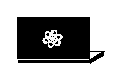
\includegraphics[scale=2.4]{Vectors/laptop_q.eps}\newline Quantum Computing}

{
\setbeamertemplate{frame footer}{\tiny{\textsuperscript{1}}}
\begin{frame}[fragile]{Classical vs. quantum bits (qubits)}

\begin{figure}
\includegraphics[scale=0.3]{MOSFET.png}
\end{figure}
\vspace{-0.3cm}
\centering{
\tiny{Source: Wikipedia}}
%metal–oxide–semiconductor field-effect transistor
\flushleft
\textbf{Classical bit:}
\begin{itemize}
\item Usually implemented through MOSFETs
\item 2 definite states ($0$,$1$)
\item Can be either $0$ OR $1$
\end{itemize}

\end{frame}
}

{
%\setbeamertemplate{frame footer}{\tiny{\textsuperscript{1}Reprinted from RF Wireless World, n.d., Retrieved December 23, 2016, from \url{http://www.rfwireless-world.com/Terminology/Difference-between-Bit-and-Qubit.html}. Copyright 2012 by RF Wireless World.}}
\begin{frame}[fragile]{Classical vs. quantum bits (qubits)}

\textbf{Quantum bit (qubit):}
\begin{itemize}
\item Can be $\ket{0}$ OR $\ket{1}$
\item But it can also be $\ket{0}$ AND $\ket{1}$ $\rightarrow$ quantum superposition
\end{itemize}

\begin{figure}
\includegraphics[scale=0.3]{qubitimplementation.jpeg}
%\caption{Example of a physical qubit.\textsuperscript{1}}
\end{figure}
\tiny{Source: RF Wireless World}

%introduce ket vectors \& superposition
%show vector representation of a qubit
\end{frame}
}

{
\setbeamertemplate{frame footer}{\tiny{}}
\begin{frame}[fragile]{A qubit}

Mathematically, the superposition of a qubit is expressed as:
\begin{equation}
\label{equ:simplequbit}
\ket{\psi} = \alpha \ket{0} + \beta \ket{1} \doteq \begin{pmatrix}\alpha\\\beta\end{pmatrix}\, ,
\end{equation}
where $\alpha, \beta \in \mathbb{C}$ and they are called amplitudes.

%$\ket{0}$ and $\ket{1}$ can be represented as the 2-D vectors:
%\begin{equation}
%\ket{0} \doteq  \begin{pmatrix}1\\0\end{pmatrix} \quad %\mathrm{and} \quad \ket{1} \doteq \begin{pmatrix}0\\1\end{pmatrix}\, .
%\end{equation}

%Substituting into Eq.~\ref{equ:simplequbit} yields the vector %representation of $\ket{\psi}$:
%\begin{equation}
%\ket{\psi} \doteq \alpha \begin{pmatrix} 1\\0 \end{pmatrix} + %\beta \begin{pmatrix}0\\1 \end{pmatrix} = \begin{pmatrix}\alpha\\\beta\end{pmatrix}\, .
%\end{equation}
The last expression is called the \textbf{amplitude vector}.
%introduce ket vectors \& superposition
%show vector representation of a qubit
\end{frame}
}

{
\setbeamertemplate{frame footer}{\tiny{\textsuperscript{1}Reprinted from Wikipedia, n.d., Retrieved September 7, 2016, from \url{https://en.wikipedia.org/wiki/Bloch_Sphere}. Copyright 2012 by Glosser.ca. Reprinted with permission.}}
\begin{frame}[fragile]{The Bloch sphere}

\begin{minipage}[c]{.5\textwidth}
		%\centering
		\hspace{2mm}
       \includegraphics[width=0.8\textwidth]{blochsphere.png}
       \captionsetup{justification=raggedright, singlelinecheck=false}
       \captionof{figure}{\footnotesize{Arbitrary two-dimensional qubit $\ket{\psi}$ visualized on the Bloch sphere\textsuperscript{1}} }
\end{minipage}%%%%%
\begin{minipage}[c][][b]{.5\textwidth}
Most general form of a 2-D qubit:
\begin{equation}
\label{equ: blochqubit}
\ket{\psi} = \alpha \ket{0} + \beta \ket{1}\, ,
\end{equation}
where $\alpha,\beta \in \mathbb{C}$.\\
\\
Can also be visualized in spherical polar coords on the unit or Bloch sphere as follows: 

\begin{equation}
\label{equ: blochqubit}
\ket{\psi} = \cos\frac{\theta}{2} \ket{0} + e^{i \phi} \sin\frac{\theta}{2} \ket{1}\, ,
\end{equation}
where $0 \leq \theta \leq \pi$ and $0 \leq \phi \leq 2\pi$
\null
\par\xdef\tpd{\the\prevdepth}
\end{minipage}

\end{frame}
}


{
\setbeamertemplate{frame footer}{\tiny{}}
\begin{frame}[fragile]{Multi-qubit systems: the power of quantum computing}

A quantum computer with $n$ qubits has $2^n$ quantum amplitudes.\\
$\rightarrow$ these amplitudes can be used to store huge amounts of information!
%\begin{itemize}
%\item It follows, that an $n$-qubit system has $2^n$ amplitudes.\\
%$\rightarrow$ can be used to store huge amounts of information!

%\item Equivalently, to simulate an $n$-qubit quantum computer one needs to store the value of all $2^n$ amplitudes:\\
%$\rightarrow$ requires $2^n\cdot 64$ classical bits of random-access memory (RAM).
%\end{itemize}

\begin{table}[H]
\begin{tabular}{C{2cm} | C{4cm} | C{4cm}}
\toprule
Qubit number & classical RAM needed & Simulation time\\\midrule
5 & 256 bytes & microseconds on smartphone \\\midrule
25 &  2 gigabytes & seconds on a laptop\\\midrule
50 & 8000 terabytes & seconds on next year's supercomputer\\\midrule
275 & number of atoms in the visible universe & age of the universe \\
\bottomrule
\end{tabular}
\end{table}

%For example:
%\begin{itemize}
%\item 25 qubits can be simulated with just 2 gigabytes of RAM.
%\item However, 50 qubits require $\sim$8000 terabytes of RAM
%\item Lastly, 275 qubits have $2^{275} \approx 6\times 10^{82}$ amplitudes which is roughly equal to the number of atoms in our universe
%\end{itemize}

\end{frame}
}

{
\setbeamertemplate{frame footer}{\tiny{}}
\begin{frame}[fragile]{State-of-the-art quantum computation}

\textbf{However}, quantum computation is cutting edge research at the frontier of supercomputing technology!\\
\vspace{0.1cm}
$\rightarrow$ State-of-the art quantum computers are complicated laboratory experiments.

\begin{minipage}[c]{0.59\textwidth}
\vspace{0.3cm}
\textbf{Current state-of-the-art:}\\
\begin{itemize}
\item IBM $\rightarrow$ \textbf{5 superconducting qubits}
\item Google $\rightarrow$ \textbf{9 superconducting qubits}
\item Weizmann Research Group in Israel\\$\rightarrow$ \textbf{8 trapped ions}
\item DWave $\rightarrow$ \textbf{1,152 qubits}\\BUT solves only a narrow class of problems
\end{itemize}
\end{minipage}%%
\begin{minipage}[c]{0.39\textwidth}
\includegraphics[scale=0.18]{ion-trap.jpg}\\
\centering
\tiny{Source: University of Innsbruck}
\end{minipage}

\end{frame}
}

{
\setbeamertemplate{frame footer}{\tiny{}}
\begin{frame}[fragile]{Motivation for this thesis research}

\begin{itemize}
\item Classical machine learning is a very applied field
\item State-of-the-art quantum computer have very small numbers of qubits
\item Thus, quantum-enhanced machine learning is almost purely theoretical
\item There have been only a handful of proof-of-principle studies in quantum-enhanced machine learning
\item Need for more proof-of-principle implementations and simulations to demonstrate the benefits of quantum computation for machine learning
\item Small machine learning problems need to be identified and implemented.
\end{itemize}

\end{frame}
}

\section{Methods}

{
\setbeamertemplate{frame footer}{\tiny{\textsuperscript{1} Screenshot taken from \url{https://quantumexperience.ng.bluemix.net/qstage/\#/editor}}}
\begin{frame}[fragile]{Methods: IBM Quantum Experience}

\begin{figure}
\includegraphics[height=0.45\textwidth]{IBMamplitudecomposer.png}
       \caption{\footnotesize{IBM's quantum composer\textsuperscript{1}} }
\end{figure}
\vspace{-5mm}
\begin{minipage}[t]{.5\textwidth}
\begin{itemize}
\item Accessible to the public
\item Allows for ideal + real simulations
\end{itemize}
\end{minipage}%%%%
\begin{minipage}[t]{.5\textwidth}
\begin{itemize}
\item 5 superconducting qubits
\item 40 gates (39 gates + 1 measurement)

\end{itemize}
\end{minipage}

\end{frame}
}

{
\setbeamertemplate{frame footer}{\tiny{}}
\begin{frame}[fragile]{Methods: Liqui$\ket{}$}

Small quantum computers can be simulated on conventional classical computers!\\
\vspace{0.5cm}
%\begin{figure}
%\includegraphics[height=0.4\textwidth]{liquidcodesnippet.png}
%\end{figure}
%\vspace{-5mm}
%\begin{minipage}[t]{.5\textwidth}
Liqui$\ket{}$...
\begin{itemize}
\item stands for Language-Integrated Quantum Operations. 
\item is a quantum simulation toolsuite written in F\# and developed by Microsoft Research.
\item allows for simulations of up to 30 qubits with 16GB RAM.
\item was used in this thesis to provide proof-of-principle simulations of quantum-enhanced machine learning algorithms.
%\end{itemize}
%\end{minipage}%%%%
%%\begin{minipage}[t]{.5\textwidth}
%\begin{itemize}
%\item 5 superconducting qubits
%\item 40 gates (39 gates + 1 measurement)

\end{itemize}
%\end{minipage}

\end{frame}
}

\section*{\protect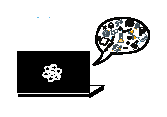
\includegraphics[scale=2.4]{Vectors/laptop_qml.eps}\newline Quantum-enhanced Machine Learning}

{
\setbeamertemplate{frame footer}{\tiny{\textsuperscript{1}}}
\begin{frame}[fragile]{Encoding classical data into amplitudes}

%There are two different ways for encoding classical data into quantum states. 
\begin{alertblock}{Data encoded into amplitudes}
k-dimensional probability vector is encoded into $log_{2}(k)$ qubits, e.g.\\ 
\vspace{2mm}
$\begin{pmatrix}
 \textcolor{blue}{0.6} \\ 
 \textcolor{emerald}{0.4}
 \end{pmatrix} \quad \rightarrow \quad \ket{n} = \sqrt{\textcolor{blue}{0.6}}\ket{0}+\sqrt{\textcolor{emerald}{0.4}}\ket{1}$\\
%\textbf{Possibility of exponential speed up}
\end{alertblock}
\vspace{0.5cm}
Schuld, Fingerhuth, and Petruccione (Manuscript in preparation) developed a new \textbf{amplitude-based} kNN algorithm.\\
$\rightarrow$ requires only a few qubits and provides great speed-up

\end{frame}
}

{
\setbeamertemplate{frame footer}{\tiny{Schuld, Fingerhuth, and Petruccione (Manuscript in preparation) Amplitude-based quantum k-nearest neighbour algorithm.}}
\begin{frame}[fragile]{The amplitude-based kNN algorithm}

\begin{enumerate}
\item $\ket{\psi_0} = \frac{1}{\sqrt{2M}}\sum_{m=1}^{M} (\ket{0}\ket{\Psi_{\tilde{x} (\star)}}+\ket{1}\ket{\Psi_{x^{m}}})\ket{y^{m}}\ket{m}$\hspace{2cm} [Initial quantum state]
\vspace{0.3cm}
\item $\ket{\psi_1} =  \frac{1}{2\sqrt{M}}\sum_{m=1}^{M} (\ket{0}[\ket{\Psi_{\tilde{x}}}+\ket{\Psi_{x^{m}}}]+\ket{1}[\ket{\Psi_{\tilde{x}}}-\ket{\Psi_{x^{m}}}])\ket{y^{m}}\ket{m}$ \hfill
[Distance computations with quantum interference]
\vspace{0.3cm}
\item $\ket{\psi_2} = \frac{1}{2\sqrt{M}}\sum_{m=1}^{M} \sum_{i=1}^{N} (\tilde{x}_i+x_i^m)\ket{0}\ket{i}\ket{y^{m}}\ket{m}$\hfill
\hspace{2cm}[Conditional measurement]
\vspace{0.3cm}
\item $\mathrm{Prob}(\ket{y^m} = \ket{1})= \sum_{m \mid y^m=1} 1 - \frac{1}{4M} \mid \tilde{x} - x^m \mid ^2$\hfill
\hspace{2cm} [Probability to measure a certain class]
\item $ y = \begin{cases}
      0, & \text{if}\ \mathrm{Prob}(\ket{y^0}) > \mathrm{Prob}(\ket{y^1}) \\
      1, & \text{if}\ \mathrm{Prob}(\ket{y^1}) > \mathrm{Prob}(\ket{y^0}) \\
      -, & \text{otherwise}
    \end{cases}$\hspace{1cm} [Classification]
\end{enumerate}
%where
%\begin{flalign}
%\ket{\Psi_{\tilde{x}}} = \sum_{i=1}^{N} \tilde{x}_i\ket{i} \quad \quad
%\ket{\Psi_{x^{m}}}	 = \sum_{i=1}^{N} x_i^m \ket{i} 
%\end{flalign}
%\begin{flalign}
%\end{flalign}
%After successful conditional measurement, the state is proportional to
%\begin{flalign}
%\end{flalign}
%Probability to measure class B:
\end{frame}
}

{
\setbeamertemplate{frame footer}{\tiny{\textsuperscript{1}}}
\begin{frame}[fragile]{Calculating distances with interference}

%\movie[width=5cm,height=3.8cm,poster,autostart]{}{interference.avi}
%\includemedia[
%  label=vidA,
%  addresource=interference.avi,
%  activate=pageopen,
%  width=5cm, height=3.8cm,
%  flashvars={
%     source=interference.mp4
%    &loop=true
%  }
%]{}{VPlayer.swf}
%\mediabutton[
%  mediacommand=vidA:playPause,
%]{\fbox{Play/Pause}}
\begin{figure}[ht]
\includegraphics[scale=0.5]{wave-interference.png}
\end{figure}
\centering
\tiny{Source: TutorVista}

\end{frame}
}

\section{Results: Amplitude-based kNN algorithm}

{
\setbeamertemplate{frame footer}{}
\begin{frame}{Simple binary classification case}

\begin{figure}
       \includegraphics[scale=0.3]{bloch3over4.png}
       \captionsetup{justification=raggedright, singlelinecheck=false}
       \captionof{figure}{\footnotesize{Simple binary classification problem of a quantum state} }
\end{figure}%%%%

\end{frame}
}

{
\setbeamertemplate{frame footer}{}
\begin{frame}{IBM's universal gate set}

\begin{figure}
\includegraphics[scale=0.45]{IBMgates.png}
       \caption{\footnotesize{IBM's universal gate set} }
\end{figure}
\vspace{10mm}
\centering{\textbf{How can we implement the amplitude-based quantum kNN algorithm with this small gate set?}}

\end{frame}
}

{
\setbeamertemplate{frame footer}{}
\begin{frame}{Results: IBM quantum computer implementation}

\begin{itemize}
\item IBM's short qubit lifetimes only allow for 40 quantum gates. 
\item IBM Quantum Experience has a very small universal gate set making it difficult to run complicated algorithms.
\item For this particular classification problem the quantum kNN algorithm requires at least 55 quantum gates.
\item Until now, it is \textbf{impossible} to solve this particular machine learning problem on IBM's actual quantum hardware!
\end{itemize}

$\rightarrow$ Need for proof-of-principle simulations with Liqui$\ket{}$ to show that the quantum algorithms work!

\end{frame}
}

{
\setbeamertemplate{frame footer}{}
\begin{frame}{Results: Liqui$\ket{}$ simulations of amplitude-based kNN algorithm}

\begin{itemize}
\item In Liqui$\ket{}$, one can simply define any quantum logic gate.
\item Large universal gate set possible!
\item No limit on the number of quantum gate slots.
\item No need to worry about qubit lifetimes.
\end{itemize}

Simulations demonstrated 100\% accuracy on the small-scale simple Bloch vector classification problem.

$\rightarrow$ The amplitude-based kNN algorithm does work as expected and is scalable!

\end{frame}
}

\section{Conclusion}

\begin{frame}{Summary}
\begin{itemize}
\item Quantum computing is at the frontier of supercomputing and bears the potential to vastly speed up classical machine learning algorithms
\item A small-scale machine learning problem was selected for implementation and simulation of an amplitude-based quantum kNN algorithm
%\item Subsequent quantum simulations established proof-of-principle of these algorithms
\item The Bloch vector classification task could not be implemented with the IBM Quantum Experience
\item Liqui$\ket{}$ simulations demonstrated 100\% classification accuracy on Bloch vector classification task
\item Open problem: How to encode arbitrary classical data into quantum amplitude distributions?
%\item \textbf{Need for better quantum compiling and more general state preparation algorithms!}
\end{itemize}
\end{frame}

\begin{frame}{Outlook}

\begin{itemize}
%\item Complexity analysis of the qubit-based kNN algorithm
%\item Classification of gaussian probability distributions
\item Finding more small-scale machine learning problems that can already be solved with quantum-enhanced machine learning algorithms
\item Last week, IBM has released the IBM Quantum Experience 2.0 which makes an actual proof-of-principle implementation feasible. (Publication in preparation)
\item Possible collaboration with the Weizmann Research Group in Israel to implement the amplitude-based kNN algorithm in their ion trap quantum computer.
\end{itemize}
\end{frame}

\begin{frame}{References}

\footnotesize{Bekkerman, R., Bilenko, M., \& Langford, J. (2011). Scaling up machine learning: Parallel and distributed
approaches. Cambridge University Press.\newline

Booth Jr, J. (2012). Quantum compiler optimizations. arXiv preprint arXiv:1206.3348.

Dawson, C. M., \& Nielsen, M. A. (2005). The Solovay-Kitaev algorithm. arXiv preprint quant-ph/0505030.\newline

IBM. (2016). What is big data? https://www-01.ibm.com/software/data/bigdata/what-is-big
-data.html. (Accessed: 2016-09-08) \newline

Jat, R. N., \& Ruhela, D. S. (2011). Comparative study of complexity of algorithms for iterative solution of non-linear equations. Journal of International Academy Of Physical Sciences, 15(4).\newline

Nielsen, M. A., \& Chuang, I. L. (2010). Quantum computation and quantum information. Cambridge University Press.}
\end{frame}

\begin{frame}[standout]
  Questions?
\end{frame}

\section{Results: Qubit-based kNN algorithm}

{
\setbeamertemplate{frame footer}{\tiny{\textsuperscript{1}}}
\begin{frame}[fragile]{}




\end{frame}
}

\appendix
{
\setbeamertemplate{frame footer}{\tiny{\textsuperscript{1}Reprinted from Wikipedia, n.d., Retrieved September 7, 2016, from \url{https://en.wikipedia.org/wiki/Bloch_Sphere}. Copyright 2012 by Glosser.ca. Reprinted with permission.}}
\begin{frame}[fragile]{Quantum Computing \& Qubits}

\begin{minipage}[c]{.5\textwidth}
		%\centering
		\hspace{2mm}
       \includegraphics[width=0.8\textwidth]{blochsphere.png}
       \captionsetup{justification=raggedright, singlelinecheck=false}
       \captionof{figure}{\footnotesize{Arbitrary two-dimensional qubit $\ket{\psi}$ visualized on the Bloch sphere\textsuperscript{1}} }
\end{minipage}%%%%%
\begin{minipage}[c][][b]{.5\textwidth}
Most general form of a 2-D qubit:
\begin{equation}
\label{equ: blochqubit}
\ket{q} = \alpha \ket{0} + \beta \ket{1}
\end{equation}
where $\alpha,\beta \in \mathbb{C}$.\\
\\
Can also be visualized in spherical polar coords on the unit or Bloch sphere as follows: 

\begin{equation}
\label{equ: blochqubit}
\ket{q} = \cos\frac{\theta}{2} \ket{0} + e^{i \phi} \sin\frac{\theta}{2} \ket{1}
\end{equation}
where $0 \leq \theta \leq \pi$ and $0 \leq \phi \leq 2\pi$
\null
\par\xdef\tpd{\the\prevdepth}
\end{minipage}


\end{frame}
}

{
\setbeamertemplate{frame footer}{\tiny{\textsuperscript{1}IBM. (2016). What is big data? https://www-01.ibm.com/software/data/bigdata/what-is-big
-data.html. (Accessed: 2016-09-08) \newline
\textsuperscript{2}Bekkerman, R., Bilenko, M., \& Langford, J. (2011). Scaling up machine learning: Parallel and distributed
approaches. Cambridge University Press.}}
\begin{frame}[fragile]{Machine Learning}
   
\begin{itemize}
	\item Approximately 2.5 quintillion (${10}^{18}$) bytes of digital data are created every day\textsuperscript{1}
	\item Need for advanced algorithms that can make sense of data content, retrieve patterns and reveal correlations $\rightarrow$ Machine learning (ML) 
	\item ML algorithms often involve
	\begin{itemize}
	\item solving large systems of linear equations
	\item inverting large matrices
	\item distance computations
	\end{itemize}
	\item Performing these computations on large data
sets gets increasingly difficult\textsuperscript{2}

%when i.e. $\mathcal{O}(input size)$ or $\mathcal{O}(input size^{k})$ for some constant k\textsuperscript{2}
%essentially manipulations on big vectors and matrices

\end{itemize}

\end{frame}
}

{
\setbeamertemplate{frame footer}{}
\begin{frame}[fragile]{Quantum Machine Learning}

\begin{enumerate}
\item ML involves manipulation of large vectors and matrices
\item Quantum mechanics is about vectors $\in$ complex Hilbert spaces
\item Quantum computers are performing linear operations on qubits
\end{enumerate}
\hspace{3mm}$\rightarrow$ Hence, we can manipulate large vectors in parallel on quantum\\ \hspace{8mm}computers\\
\vspace{3mm}
\centering{\textcolor{orange}{So can we use QC to improve classical ML algorithms??}}
\vspace{3mm}
\begin{itemize}
\item Classical ML is a very practical topic\\
\item BUT, QML has been of almost entirely theoretical nature
\end{itemize}
\end{frame}
}

{
\setbeamertemplate{frame footer}{}
\begin{frame}[fragile]{Quantum data encoding}
 
There are two fundamentally different ways for state preparation:

\begin{alertblock}{Data encoded into qubits}
%speed-up not very clear since the \# of qubits increases linearly with the \# of classical bits
k-dimensional probability vector requires $4k$ classical bits which are encoded one-to-one into $4k$ qubits, e.g.\\
\vspace{2mm}
$\begin{pmatrix}
 \textcolor{blue}{0.6} \\ 
 \textcolor{emerald}{0.4}
 \end{pmatrix}*10 \rightarrow \begin{pmatrix}
 \textcolor{blue}{6} \\ 
 \textcolor{emerald}{4}
 \end{pmatrix} \rightarrow \begin{pmatrix}
 \textcolor{blue}{0110} \\ 
 \textcolor{emerald}{0100}
 \end{pmatrix} \rightarrow n=\textcolor{blue}{0110}\textcolor{emerald}{0100} \rightarrow \ket{n} = \ket{\textcolor{blue}{0110}\textcolor{emerald}{0100}}$\\
%\textbf{Only slight speed up possible}
\end{alertblock}
\vspace{3mm}
\begin{alertblock}{\textcolor{gray}{Data encoded into amplitudes}}
\textcolor{gray}{k-dimensional probability vector is encoded into $log_{2}(k)$ qubits, e.g.\\ 
\vspace{2mm}
$\begin{pmatrix}
 0.6 \\ 
 0.4
 \end{pmatrix} \quad \rightarrow \quad \ket{n} = \sqrt{0.6}\ket{0}+\sqrt{0.4}\ket{1}$\\
%\textbf{Possibility of exponential speed up}
}
\end{alertblock}

\end{frame}
}

{
\setbeamertemplate{frame footer}{}
\begin{frame}[fragile]{Quantum data encoding}
 
There are two fundamentally different ways for state preparation:

\begin{alertblock}{\textcolor{gray}{Data encoded into qubits}}
%speed-up not very clear since the \# of qubits increases linearly with the \# of classical bits
\textcolor{gray}{k-dimensional probability vector requires $4k$ classical bits which are encoded one-to-one into $4k$ qubits, e.g.\\
\vspace{2mm}
$\begin{pmatrix}
 0.6 \\ 
 0.4
 \end{pmatrix}*10 \rightarrow \begin{pmatrix}
 6 \\ 
 4
 \end{pmatrix} \rightarrow \begin{pmatrix}
 0110 \\ 
 0100
 \end{pmatrix} \rightarrow n=01100100 \rightarrow \ket{n} = \ket{01100100}$\\
%\textbf{Only slight speed up possible}
}
\end{alertblock}  
\vspace{3mm}
\begin{alertblock}{Data encoded into amplitudes}
k-dimensional probability vector is encoded into $log_{2}(k)$ qubits, e.g.\\ 
\vspace{2mm}
$\begin{pmatrix}
 \textcolor{blue}{0.6} \\ 
 \textcolor{emerald}{0.4}
 \end{pmatrix} \quad \rightarrow \quad \ket{n} = \sqrt{\textcolor{blue}{0.6}}\ket{0}+\sqrt{\textcolor{emerald}{0.4}}\ket{1}$\\
%\textbf{Possibility of exponential speed up}
\end{alertblock}


\end{frame}
}

{
\setbeamertemplate{frame footer}{\tiny{\textsuperscript{1}Reprinted from GitHub, Burton de Wilde, Retrieved September 13, 2016, from http://bdewilde.github.io/blog/
blogger/2012/10/26/classification-of-hand-written-digits-3/. Copyright 2012 by Burton de Wilde. Reprinted with
permission.}}
\begin{frame}[fragile]{Classical k-nearest neighbour}
 

\centering{
- kNN is a non-parametric classifier\\
- $k$ is a positive integer, usually chosen small}

\begin{minipage}[t]{.35\textwidth}
Given training data set:\\
${D}_{T}$ = ${v}_{0}, {v}_{1},..,{v}_{10}$ \\
$v_{i} \in$ \{$A$, $B$\}

\end{minipage}%%%
\begin{minipage}[t]{.65\textwidth}
Given a new vector $\tilde{x}$ (red star):\\
- consider $k$ nearest neighbours\\
- classify $\tilde{x}$, based on majority vote, as $A$ or $B$
\end{minipage}

\begin{figure}
       \includegraphics[width=0.5\textwidth]{knn-concept.png}
      \caption{\footnotesize{Visualization of a kNN classifier\footnotemark[1]}}
\end{figure}
 
\end{frame}
}


%\section{Amplitude-based kNN algorithm}
{
\setbeamertemplate{frame footer}{\vspace{-2mm}\tiny{Maria Schuld (2016), unpublished}}
\begin{frame}{The algorithm}

\begin{equation}
\frac{1}{\sqrt{2M}}\sum_{m=1}^{M} (\textcolor{emerald}{\ket{0}}\ket{\textcolor{red}{\Psi_{\tilde{x}} (\star)}}+\textcolor{emerald}{\ket{1}}\ket{\textcolor{darkyellow}{\Psi}_{\textcolor{purple}{x^{m}}}})\ket{y^{m}(\textcolor{darkyellow}{A} \ or \ \textcolor{purple}{B})}\ket{m}
\end{equation}
where
\begin{equation}
\ket{\textcolor{red}{\Psi_{\tilde{x}} (\star)}} = \sum_{i=1}^{N} \textcolor{red}{\tilde{x}_i}\ket{i} \quad \quad
\ket{\textcolor{darkyellow}{\Psi}_{\textcolor{purple}{x^{m}}}}	 = \sum_{i=1}^{N} \textcolor{darkyellow}{x}\textcolor{purple}{_i^m} \ket{i} 
\end{equation}

\begin{equation}
e.g. \quad \begin{pmatrix}
 \textcolor{blue}{0.6} \\ 
 \textcolor{emerald}{0.4}
 \end{pmatrix} \quad \rightarrow \quad \ket{n} =  \sqrt{\textcolor{blue}{0.6}}\ket{0}+\sqrt{\textcolor{emerald}{0.4}}\ket{1}
\end{equation}

\begin{figure}
       \includegraphics[scale=.25]{knn-concept.png}
      \caption{\footnotesize{Visualization of a kNN classifier\footnotemark[1]}}
\end{figure}

\end{frame}
}

{
\setbeamertemplate{frame footer}{\vspace{-2mm}\tiny{Maria Schuld (2016), unpublished}}
\begin{frame}{The algorithm}

Applying the \textbf{Hadamard gate} interferes the input and the training vectors:

\begin{equation}
\frac{1}{2\sqrt{M}}\sum_{m=1}^{M} (\textcolor{emerald}{\ket{0}}[\ket{\textcolor{red}{\Psi_{\tilde{x}}}}+\ket{\textcolor{darkyellow}{\Psi}_{\textcolor{purple}{x^{m}}}}]+\textcolor{emerald}{\ket{1}}[\ket{\textcolor{red}{\Psi_{\tilde{x}}}}-\ket{\textcolor{darkyellow}{\Psi}_{\textcolor{purple}{x^{m}}}}])\ket{y^{m}(\textcolor{darkyellow}{A} \ or \ \textcolor{purple}{B})}\ket{m}
\end{equation}

$\rightarrow$ Perform \textbf{conditional measurement} on ancilla qubit.\\
Successful if $\ket{0}$ state is measured.
\end{frame}
}

{
\setbeamertemplate{frame footer}{\vspace{-2mm}\tiny{Maria Schuld (2016), unpublished}}
\begin{frame}{The algorithm}

After successful conditional measurement, the state is proportional to
\begin{equation}
\frac{1}{2\sqrt{M}}\sum_{m=1}^{M} \sum_{i=1}^{N} (\textcolor{red}{\tilde{x}_i}+\textcolor{darkyellow}{x}\textcolor{purple}{_i^m})\ket{0}\ket{i}\ket{y^{m}(\textcolor{darkyellow}{A} \ or \ \textcolor{purple}{B})}\ket{m}
\end{equation}

Probability to measure class B:
\begin{equation}
p(\ket{y^m} = \ket{1(\textcolor{purple}{B})})= \sum_{m \mid y^m=1(\textcolor{purple}{B})} 1 - \frac{1}{4M} \mid \textcolor{red}{\tilde{x}} - \textcolor{purple}{x^m} \mid ^2
\end{equation}
	\metroset{block=fill}
	\begin{alertblock}{Overall algorithmic complexity}
	\centering
	$\mathcal{O}(\frac{1}{p_{acc}})$ where $p_{acc}$ is the probability of measuring ancilla in the $\ket{0}$ state
	\end{alertblock}
\end{frame}
}


{
\setbeamertemplate{frame footer}{}
\begin{frame}{Simple binary classification case}

\begin{minipage}[c]{.4\textwidth}
		%\centering
		\hspace{-7mm}
       \includegraphics[width=1.1\textwidth]{bloch3over4.png}
       \captionsetup{justification=raggedright, singlelinecheck=false}
       \captionof{figure}{\footnotesize{Simple binary classification problem of a quantum state} }
\end{minipage}%%%%
\begin{minipage}[c][][b]{.6\textwidth}
\scriptsize{
\begin{equation}
\frac{1}{\sqrt{2M}}\sum_{m=1}^{M} (\textcolor{emerald}{\ket{0}}\ket{\textcolor{red}{\Psi_{\tilde{x}} (\star)}}+\textcolor{emerald}{\ket{1}}\ket{\textcolor{darkyellow}{\Psi}_{\textcolor{purple}{x^{m}}}})\ket{y^{m}(\textcolor{darkyellow}{A} \ or \ \textcolor{purple}{B})}\ket{m}
\end{equation}}
Procedure to load the input vector $\tilde{x}$:
\begin{equation}
\ket{\Psi_0} = \frac{1}{2}\sum_{m=1}^{2} (\textcolor{emerald}{\ket{0}}\ket{0}+\textcolor{emerald}{\ket{1}}\ket{0})\ket{y^{m}}\ket{m}
\end{equation}
Apply controlled rotation $_0^1CR_y(\frac{\pi}{4})$ s.t.
\begin{equation}
_0^1CR_y(\frac{\pi}{4})\ket{\Psi_0} = \ket{\Psi_1} = \frac{1}{2}\sum_{m=1}^{2} (\textcolor{emerald}{\ket{0}}\ket{0}+\textcolor{emerald}{\ket{1}}\ket{\textcolor{red}{\Psi_{\tilde{x}}}})\ket{y^{m}}\ket{m}
\end{equation}
Flip the ancilla qubit in the first register
\begin{equation}
(X\otimes\mathds{1}\otimes\mathds{1}\otimes\mathds{1})\ket{\Psi_1} = \ket{\Psi_2} = \frac{1}{2}\sum_{m=1}^{2} (\textcolor{emerald}{\ket{0}}\ket{\textcolor{red}{\Psi_{\tilde{x}}}}+\textcolor{emerald}{\ket{1}}\ket{0})\ket{y^{m}}\ket{m}
\end{equation}
\null
\par\xdef\tpd{\the\prevdepth}
\end{minipage}

	%\metroset{block=fill}
	%\begin{alertblock}{Algorithmic complexity}
	%\centering
	%$\mathcal{O}(\frac{1}{p_{acc}})$
	%\end{alertblock}

\end{frame}
}

{
\setbeamertemplate{frame footer}{}
\begin{frame}{Implementation with IBM's quantum computer}

\begin{figure}
\includegraphics[height=0.5\textwidth]{IBMamplitudecomposer.png}
       \caption{\footnotesize{IBM's quantum composer} }
\end{figure}
\vspace{-5mm}
\begin{minipage}[t]{.5\textwidth}
\begin{itemize}
\item Accessible to the public
\item Allows for ideal + real simulations
\end{itemize}
\end{minipage}%%%%
\begin{minipage}[t]{.5\textwidth}
\begin{itemize}
\item 5 superconducting qubits
\item 40 gates (39 gates + 1 measurement)

\end{itemize}
\end{minipage}
\end{frame}
}

{
\setbeamertemplate{frame footer}{}
\begin{frame}{IBM's universal gate set}

\begin{figure}
\includegraphics[scale=0.45]{IBMgates.png}
       \caption{\footnotesize{IBM's universal gate set} }
\end{figure}
\vspace{10mm}
\centering{\textbf{How can we implement the $_0^1CR_y(\frac{\pi}{4})$ gate?}}

\end{frame}
}

{
\setbeamertemplate{frame footer}{}
\begin{frame}{Liqui$\ket{}$ simulations}
	
Currently impossible to implement the quantum algorithm on IBM's quantum computer!
$\rightarrow$ can only simulate it with i.e. Liqui$\ket{}$

In Liqui$\ket{}$ we can directly implement the controlled $R_y$ rotation!

%Could you also show what happens if I use approximated gate sequences?	
%Run the command mono Liquid.exe "__BinaryAmplitudeKNN(10000)" in a terminal

\end{frame}
}

\section{Conclusion}

\begin{frame}{Summary}
\begin{itemize}
\item Initial state preparation is non-trivial! (even for very simple examples)
\item In this case, state preparation dominates the overall algorithmic complexity
\item Solovay-Kitaev yields long gate sequences for good approximations
\item Some universal gate sets are only useful when combined with long qubit lifetimes
\item \textbf{Need for better quantum compiling and more general state preparation algorithms!}
\end{itemize}
\end{frame}

\begin{frame}{Taking it further}

\begin{itemize}
\item Complexity analysis of the qubit-based kNN algorithm
\item Classification of gaussian probability distributions
\item Implementing more general state preparation algorithms
\item Waiting for IBM QASM 2.0 ...
\end{itemize}
\end{frame}

\begin{frame}{References}

\footnotesize{Bekkerman, R., Bilenko, M., \& Langford, J. (2011). Scaling up machine learning: Parallel and distributed
approaches. Cambridge University Press.\newline

Booth Jr, J. (2012). Quantum compiler optimizations. arXiv preprint arXiv:1206.3348.

Dawson, C. M., \& Nielsen, M. A. (2005). The Solovay-Kitaev algorithm. arXiv preprint quant-ph/0505030.\newline

IBM. (2016). What is big data? https://www-01.ibm.com/software/data/bigdata/what-is-big
-data.html. (Accessed: 2016-09-08) \newline

Jat, R. N., \& Ruhela, D. S. (2011). Comparative study of complexity of algorithms for iterative solution of non-linear equations. Journal of International Academy Of Physical Sciences, 15(4).\newline

Nielsen, M. A., \& Chuang, I. L. (2010). Quantum computation and quantum information. Cambridge University Press.}
\end{frame}

\begin{frame}[standout]
  Questions?
\end{frame}

{
\setbeamertemplate{frame footer}{\vspace{-2mm}\tiny{Chuang I. (2003) MIT Lecture 19: How to Build Your Own Quantum Computer}}
\begin{frame}[fragile]{Backup slide: Qubit decoherence times}

We expect exponential decay:
\begin{equation}
e^{−t/T_i}
\end{equation}

\begin{block}{$T_1$: Longitudinal coherence time (amplitude damping)}

- Prepare $\ket{0}$ state\\
- Apply the X (NOT) gate s.t. qubit is in $\ket{1}$ state\\
- Wait for time $t$\\
- Measure the probability of being in $\ket{1}$ state

\end{block}
\begin{block}{$T_2$: Transversal coherence time (phase damping)}

- Prepare $\ket{0}$ state\\
- Apply Hadamard $\rightarrow \quad \frac{\ket{0}+\ket{1}}{\sqrt{2}}$\\
- Wait for time $t$\\
- Apply Hadamard again\\
- Measure the probability of being in $\ket{0}$ state\\

We expect this probability to go to 0.5 $\rightarrow$ qubit lost quantum behaviour
\end{block}

\end{frame}
}
{
\setbeamertemplate{frame footer}{\tiny{\textsuperscript{1}Li, Z., Liu, X., Xu, N., \& Du, J. (2015). Experimental realization of a quantum support vector machine. Physical Review Letters, 114 (14), 1–5. doi: 10.1103/PhysRevLett.114.140504 \newline\textsuperscript{2}Cai, X. D., Wu, D., Su, Z. E., Chen, M. C., Wang, X. L., Li, L., . . . Pan, J. W. (2015). Entanglement-
based machine learning on a quantum computer. Physical Review Letters, 114 (11), 1–5. doi:10.1103/PhysRevLett.114.110504 \newline\textsuperscript{3}Ristè, D., da Silva, M. P., Ryan, C. A., Cross, A. W., Smolin, J. A., Gambetta, J. M., . . . Johnson,
B. R. (2015). Demonstration of quantum advantage in machine learning. arXiv:1512.06069 , 1–12.
Retrieved from http://arxiv.org/abs/1512.06069 }}
\begin{frame}[fragile]{Backup Slide II: Experimental realizations}


Only few experimental verifications of QML algorithms:

- Li, Liu, Xu, and Du (2015) successfully distinguished a handwritten six from a nine using a
quantum support vector machine on a four-qubit nuclear magnetic resonance test bench\textsuperscript{1}

- Cai et al. (2015) were first to experimentally demonstrate quantum machine learning on a photonic QC and showed that the distance between two vectors and their inner product can indeed be computed quantum
mechanically\textsuperscript{2}

- Ristè et al. (2015) solved a learning parity problem with five superconducting qubits and found that a quantum advantage can already be observed in non error-corrected systems\textsuperscript{3}


%Explain the experimental results that have been shown so far. Outline problems with non-error corrected qubits, gate times and small qubit numbers.

%> only proof-of-concept so far
%little is known about full procedure from crude data to final classification

\end{frame}
}

{
\setbeamertemplate{frame footer}{}
\begin{frame}[fragile]{Machine Learning}
   
Machine learning can be subdivided into three major fields.

\metroset{block=fill}

\begin{alertblock}{Supervised ML}
- Based on \emph{input} and \emph{output} data\\
\centering{
"I know how to classify this data but I need the algorithm to do the computations for me."}
\end{alertblock}

\begin{exampleblock}{Unsupervised ML}
- Based on \emph{input} data only\\
\centering{
"I have no clue how to classify this data, can the algorithm create a classifier for me?"}
\end{exampleblock}

\begin{block}{Reinforcement learning}
- Based on \emph{input} data only\\
\centering{
"I have no clue how to classify this data, can the algorithm classify this data and I'll give it a reward if it's correct or I'll punish it if it's not."}
\end{block}

\end{frame}
}

{
\setbeamertemplate{frame footer}{}
\begin{frame}[fragile]{Machine Learning}
   
Machine learning can be subdivided into three major fields.

\metroset{block=fill}

\begin{alertblock}{Supervised ML}
- Based on \emph{input} and \emph{output} data\\
\centering{
"I know how to classify this data but I need the algorithm to do the computations for me."}
\end{alertblock}

\begin{exampleblock}{\textcolor{gray}{Unsupervised ML}}
\color{gray}
- Based on \emph{input} data only\\
\centering{
"I have no clue how to classify this data, can the algorithm create a classifier for me?"}
\end{exampleblock}

\begin{block}{\textcolor{gray}{Reinforcement learning}}
\color{gray}
- Based on \emph{input} data only\\
\centering{
"I have no clue how to classify this data, can the algorithm classify this data and I'll give it a reward if it's correct or I'll punish it if it's not."}
\end{block}

\end{frame}
}

{
\setbeamertemplate{frame footer}{}
\begin{frame}{Liqui$\ket{}$ simulations: Taking it further}

\begin{figure}
\includegraphics[scale=0.35]{cube_notdiffused.png}
       \caption{\footnotesize{Representation of hamming distance on 3D cube} }
\end{figure}
\end{frame}
}

{
\setbeamertemplate{frame footer}{}
\begin{frame}{Liqui$\ket{}$ simulations: Taking it further}

Applying the following matrix
\begin{equation}
\begin{pmatrix}
 \sqrt{\delta} & 1-\sqrt{\delta} \\ 
 1-\sqrt{\delta} & -\sqrt{\delta}
 \end{pmatrix}
\end{equation}
to all qubits in the data register leads to a gaussian distribution over the "Hamming distance" cube:

\begin{figure}
\includegraphics[scale=0.2]{4qubitdiffusion.png}
       \caption{\footnotesize{Gaussian diffusion of a quantum state} }
\end{figure}

\end{frame}
}

{
\setbeamertemplate{frame footer}{}
\begin{frame}{Liqui$\ket{}$ simulations: Taking it further}

\begin{figure}
\includegraphics[scale=0.33]{cube_diffused.png}
       \caption{\footnotesize{Representation of gaussian diffusion on 3D cube} }
\end{figure}
\end{frame}
}

{
\setbeamertemplate{frame footer}{}
\begin{frame}{Liqui$\ket{}$ simulations: Taking it further}

\begin{figure}
\includegraphics[scale=0.33]{4d_hypercube.png}
       \caption{\footnotesize{Representation of gaussian diffusion on 3D cube} }
\end{figure}
\end{frame}
}

\begin{frame}[allowframebreaks]{Backup slide II}

  \bibliography{demo}
  \bibliographystyle{abbrv}

\end{frame}

\section{Qubit-based kNN quantum algorithm}

{
\setbeamertemplate{frame footer}{References go here}
\begin{frame}[fragile]{Typography}
      \begin{verbatim}The theme provides sensible defaults to
\emph{emphasize} text, \alert{accent} parts
or show \textbf{bold} results.\end{verbatim}

  \begin{center}becomes\end{center}

  The theme provides sensible defaults to \emph{emphasize} text,
  \alert{accent} parts or show \textbf{bold} results.
\end{frame}
}

{
\setbeamertemplate{frame footer}{References go here}
\begin{frame}{Font feature test}
  \begin{itemize}
    \item Regular
    \item \textit{Italic}
    \item \textsc{SmallCaps}
    \item \textbf{Bold}
    \item \textbf{\textit{Bold Italic}}
    \item \textbf{\textsc{Bold SmallCaps}}
    \item \texttt{Monospace}
    \item \texttt{\textit{Monospace Italic}}
    \item \texttt{\textbf{Monospace Bold}}
    \item \texttt{\textbf{\textit{Monospace Bold Italic}}}
  \end{itemize}
\end{frame}
}

\begin{frame}{Lists}
  \begin{columns}[T,onlytextwidth]
    \column{0.33\textwidth}
      Items
      \begin{itemize}
        \item Milk \item Eggs \item Potatos
      \end{itemize}

    \column{0.33\textwidth}
      Enumerations
      \begin{enumerate}
        \item First, \item Second and \item Last.
      \end{enumerate}

    \column{0.33\textwidth}
      Descriptions
      \begin{description}
        \item[PowerPoint] Meeh. \item[Beamer] Yeeeha.
      \end{description}
  \end{columns}
\end{frame}
\begin{frame}{Animation}
  \begin{itemize}[<+- | alert@+>]
    \item \alert<4>{This is\only<4>{ really} important}
    \item Now this
    \item And now this
  \end{itemize}
\end{frame}
\begin{frame}{Figures}
  \begin{figure}
    \newcounter{density}
    \setcounter{density}{20}
    \begin{tikzpicture}
      \def\couleur{alerted text.fg}
      \path[coordinate] (0,0)  coordinate(A)
                  ++( 90:5cm) coordinate(B)
                  ++(0:5cm) coordinate(C)
                  ++(-90:5cm) coordinate(D);
      \draw[fill=\couleur!\thedensity] (A) -- (B) -- (C) --(D) -- cycle;
      \foreach \x in {1,...,40}{%
          \pgfmathsetcounter{density}{\thedensity+20}
          \setcounter{density}{\thedensity}
          \path[coordinate] coordinate(X) at (A){};
          \path[coordinate] (A) -- (B) coordinate[pos=.10](A)
                              -- (C) coordinate[pos=.10](B)
                              -- (D) coordinate[pos=.10](C)
                              -- (X) coordinate[pos=.10](D);
          \draw[fill=\couleur!\thedensity] (A)--(B)--(C)-- (D) -- cycle;
      }
    \end{tikzpicture}
    \caption{Rotated square from
    \href{http://www.texample.net/tikz/examples/rotated-polygons/}{texample.net}.}
  \end{figure}
\end{frame}
\begin{frame}{Tables}
  \begin{table}
    \caption{Largest cities in the world (source: Wikipedia)}
    \begin{tabular}{lr}
      \toprule
      City & Population\\
      \midrule
      Mexico City & 20,116,842\\
      Shanghai & 19,210,000\\
      Peking & 15,796,450\\
      Istanbul & 14,160,467\\
      \bottomrule
    \end{tabular}
  \end{table}
\end{frame}
\begin{frame}{Blocks}
  Three different block environments are pre-defined and may be styled with an
  optional background color.

  \begin{columns}[T,onlytextwidth]
    \column{0.5\textwidth}
      \begin{block}{Default}
        Block content.
      \end{block}

      \begin{alertblock}{Alert}
        Block content.
      \end{alertblock}

      \begin{exampleblock}{Example}
        Block content.
      \end{exampleblock}

    \column{0.5\textwidth}

      \metroset{block=fill}

      \begin{block}{Default}
        Block content.
      \end{block}

      \begin{alertblock}{Alert}
        Block content.
      \end{alertblock}

      \begin{exampleblock}{Example}
        Block content.
      \end{exampleblock}

  \end{columns}
\end{frame}
\begin{frame}{Math}
  \begin{equation*}
    e = \lim_{n\to \infty} \left(1 + \frac{1}{n}\right)^n
  \end{equation*}
\end{frame}
\begin{frame}{Line plots}
  \begin{figure}
    \begin{tikzpicture}
      \begin{axis}[
        mlineplot,
        width=0.9\textwidth,
        height=6cm,
      ]

        \addplot {sin(deg(x))};
        \addplot+[samples=100] {sin(deg(2*x))};

      \end{axis}
    \end{tikzpicture}
  \end{figure}
\end{frame}
\begin{frame}{Bar charts}
  \begin{figure}
    \begin{tikzpicture}
      \begin{axis}[
        mbarplot,
        xlabel={Foo},
        ylabel={Bar},
        width=0.9\textwidth,
        height=6cm,
      ]

      \addplot plot coordinates {(1, 20) (2, 25) (3, 22.4) (4, 12.4)};
      \addplot plot coordinates {(1, 18) (2, 24) (3, 23.5) (4, 13.2)};
      \addplot plot coordinates {(1, 10) (2, 19) (3, 25) (4, 15.2)};

      \legend{lorem, ipsum, dolor}

      \end{axis}
    \end{tikzpicture}
  \end{figure}
\end{frame}
\begin{frame}{Quotes}
  \begin{quote}
    Veni, Vidi, Vici
  \end{quote}
\end{frame}

{
\setbeamertemplate{frame footer}{\tiny{\textsuperscript{1}}}
\begin{frame}[fragile]{Supervised machine learning: concrete example}


\begin{minipage}[c]{0.49\textwidth}
\begin{tabular}{| C{0.45cm} | C{1cm} |C{1.4cm} |}
    \toprule
      ID & Colour & Class label\\
     \midrule
      1 & \cellcolor{red1} & red \\\midrule
      2 &\cellcolor{red2} & red \\\midrule
      3 & \cellcolor{red3} & red \\\midrule\midrule
      4 & \cellcolor{blue1} & blue \\\midrule
      5 & \cellcolor{blue2} & blue \\\midrule
      6 & \cellcolor{blue3} & blue \\
     \bottomrule
   \end{tabular}
   \captionsetup{justification=raggedright, singlelinecheck=false}
   \captionof{table}{Example training dataset.}
\end{minipage}%%%
\begin{minipage}[c]{0.49\textwidth}
\centering
    \begin{tabular}{| C{0.45cm} | C{1cm} |C{1.4cm}|}
    \toprule
      ID & Colour & Class label \\
      \midrule
       1 & \cellcolor{inputred1} &  ?\\\midrule
      
       2 & \cellcolor{inputblue1} & ? \\
      \bottomrule
    \end{tabular}
    \captionof{table}{Example input dataset.}
\end{minipage}

%The machine learning algorithm should approximate the function $f$ such that it can predict the output $o$ for a new unknown input $\tilde{x}$:
%\begin{equation}
%f(\tilde{x}) = ?\, .
%\end{equation}

\end{frame}
}



{
\setbeamertemplate{frame footer}{\tiny{\textsuperscript{1}}}
\begin{frame}[fragile]{Classical $k$-nearest neighbour}

\metroset{block=fill}

\begin{alertblock}{Transferring the colours into vectors}
In the case of 9-bit RGB colours:\\
\centering{
\textcolor{red}{000} \textcolor{green}{000} \textcolor{blue}{000}}\\
3 bits for red, 3 bits for green and 3 bits for blue.
%\begin{equation}
%\begin{pmatrix}
%\textcolor{red}{red\quad content}\\ \textcolor{green}{green\quad content} \\ %\textcolor{blue}{blue\quad content}
%\end{pmatrix} = \begin{pmatrix}
%7 \\ 0 \\ 0
%\end{pmatrix}
%\end{equation}
\begin{equation}
\begin{pmatrix}
\textcolor{red}{red\quad content}\\ \cancel{\textcolor{green}{green\quad content}} \\ \textcolor{blue}{blue\quad content}
\end{pmatrix} = \begin{pmatrix}
7 \\ \cancel{0} \\ 0
\end{pmatrix} \equiv \begin{pmatrix}
7 \\ 0
\end{pmatrix}
\end{equation}
\end{alertblock}

\centering
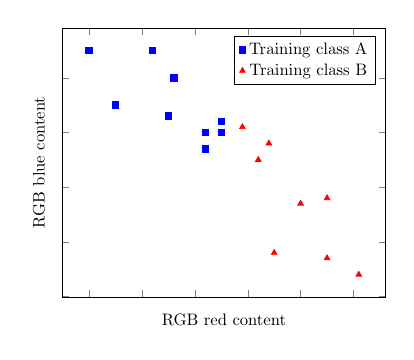
\begin{tikzpicture}[scale=0.6]
\begin{axis}[legend pos=north east,
ylabel={RGB blue content},
      xlabel={RGB red content},
      yticklabels={,,},
      xticklabels={,,},
      scatter/classes={ a={mark=square*,blue}, b={mark=triangle*,red}, c={mark=diamond*,draw=black}}] \addplot[scatter,only marks, scatter src=explicit symbolic] table[meta=label] {
x y label
0.15 -0.15 a
0.25 -0.17 a
0.26 -0.1 a
0.22 -0.05 a

0.35 -0.18 a
0.32 -0.2 a
0.32 -0.23 a
0.35 -0.2 a
0.1 -0.05 a
0.42 -0.25 b
0.44 -0.22 b
0.39 -0.19 b

0.45 -0.42 b
0.55 -0.32 b

0.61 -0.46 b
0.5 -0.33 b
0.55 -0.43 b
};
\addlegendentry{Training class A}
\addlegendentry{Training class B}
%\addlegendentry{Input vector}
\end{axis}
\end{tikzpicture}



\end{frame}
}

{
\setbeamertemplate{frame footer}{\tiny{\textsuperscript{1}}}
\begin{frame}[fragile]{Classical $k$-nearest neighbour}

\centering{
- kNN is a non-parametric classifier\\
- $k$ is a positive integer, usually chosen small}

\begin{minipage}[t]{.32\textwidth}
Given training dataset:\\
${D}_{T}$ = ${v}_{0}, {v}_{1},..,{v}_{16}$ \\
$v_{i} \in$ \{$red$, $blue$\}
\end{minipage}
\hspace{0.2cm}
\begin{minipage}[t]{.53\textwidth}
Given a new vector $\tilde{x}$ (black halfcircle):\\
- consider $k$ nearest neighbours\\
- classify $\tilde{x}$, based on majority vote,\\as \emph{red} or \emph{blue}
\end{minipage}

\begin{minipage}[c]{0.45\textwidth}
\centering
$k = 3$\\
\vspace{0.1cm}
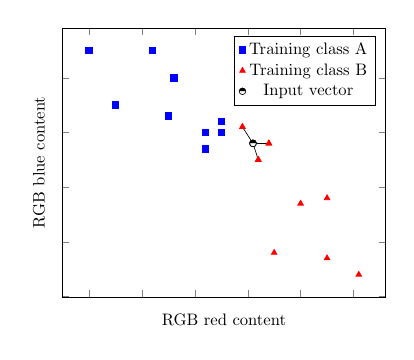
\begin{tikzpicture}[scale=0.6]
\begin{axis}[legend pos=north east,
ylabel={RGB blue content},
      xlabel={RGB red content},
 yticklabels={,,},
      xticklabels={,,},
			scatter/classes={
			a={mark=square*,blue}, 												b={mark=triangle*,red}, 											c={mark=halfcircle*,draw=black}}]
			\addplot[scatter,only marks, scatter src=explicit symbolic]
table[meta=label] {
x y label
0.15 -0.15 a
0.25 -0.17 a
0.26 -0.1 a
0.22 -0.05 a
0.35 -0.18 a
0.32 -0.2 a
0.32 -0.23 a
0.35 -0.2 a
0.1 -0.05 a
0.42 -0.25 b
0.44 -0.22 b
0.39 -0.19 b
0.45 -0.42 b
0.55 -0.32 b
0.61 -0.46 b
0.5 -0.33 b
0.55 -0.43 b
0.41 -0.22 c
};
\addplot[scatter, scatter src=explicit symbolic]
table[meta=label] {
x y label
0.42 -0.25 b
0.41 -0.22 c
};
\addplot[scatter, scatter src=explicit symbolic]
table[meta=label] {
x y label
0.44 -0.22 b
0.41 -0.22 c
};
\addplot[scatter, scatter src=explicit symbolic]
table[meta=label] {
x y label
0.39 -0.19 b
0.41 -0.22 c
};
\addlegendentry{Training class A}
\addlegendentry{Training class B}
\addlegendentry{Input vector}
\end{axis}
\end{tikzpicture}
Classification $\rightarrow$ \textbf{\textcolor{red}{RED}}
\end{minipage}
\begin{minipage}[c]{0.45\textwidth}
\centering
$k = 7$\\
\vspace{0.1cm}
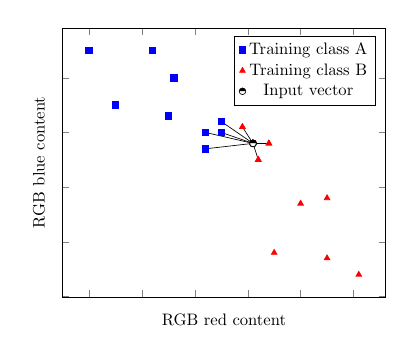
\begin{tikzpicture}[scale=0.6]
\begin{axis}[legend pos=north east,
 ylabel={RGB blue content},
      xlabel={RGB red content},
 yticklabels={,,},
      xticklabels={,,},
			scatter/classes={
			a={mark=square*,blue}, 												b={mark=triangle*,red}, 											c={mark=halfcircle*,draw=black}}]
			\addplot[scatter,only marks, scatter src=explicit symbolic]
table[meta=label] {
x y label
0.15 -0.15 a
0.25 -0.17 a
0.26 -0.1 a
0.22 -0.05 a
0.35 -0.18 a
0.32 -0.2 a
0.32 -0.23 a
0.35 -0.2 a
0.1 -0.05 a
0.42 -0.25 b
0.44 -0.22 b
0.39 -0.19 b
0.45 -0.42 b
0.55 -0.32 b
0.61 -0.46 b
0.5 -0.33 b
0.55 -0.43 b
0.41 -0.22 c
};
\addplot[scatter, scatter src=explicit symbolic]
table[meta=label] {
x y label
0.35 -0.18 a
0.41 -0.22 c
};
\addplot[scatter, scatter src=explicit symbolic]
table[meta=label] {
x y label
0.32 -0.2 a
0.41 -0.22 c
};
\addplot[scatter, scatter src=explicit symbolic]
table[meta=label] {
x y label
0.32 -0.23 a
0.41 -0.22 c
};
\addplot[scatter, scatter src=explicit symbolic]
table[meta=label] {
x y label
0.35 -0.2 a
0.41 -0.22 c
};
\addplot[scatter, scatter src=explicit symbolic]
table[meta=label] {
x y label
0.42 -0.25 b
0.41 -0.22 c
};
\addplot[scatter, scatter src=explicit symbolic]
table[meta=label] {
x y label
0.44 -0.22 b
0.41 -0.22 c
};
\addplot[scatter, scatter src=explicit symbolic]
table[meta=label] {
x y label
0.39 -0.19 b
0.41 -0.22 c
};
\addlegendentry{Training class A}
\addlegendentry{Training class B}
\addlegendentry{Input vector}
\end{axis}
\end{tikzpicture}
Classification $\rightarrow$ \textbf{\textcolor{blue}{BLUE}}
\end{minipage}
\end{frame}
}


{
\setbeamertemplate{frame footer}{\tiny{\textsuperscript{1}}}
\begin{frame}[fragile]{Single-qubit quantum logic gates}

\begin{minipage}[c]{0.49\textwidth}
\centering
\includegraphics[scale=0.18]{not_gate_c.png}
\end{minipage}%%%
\begin{minipage}[c]{0.49\textwidth}
\centering
\includegraphics[scale=0.1]{xcircuit.png}
\end{minipage}
\vspace{0.5cm}

Any single-qubit quantum logic gates can be represented by a unitary $2\times 2$ matrix whose action on a qubit is defined as:
\begin{equation}
\label{equ:unitarytransformation}
U \ket{\psi} \doteq \begin{pmatrix}
 a & b \\ 
 c & d
 \end{pmatrix} \begin{pmatrix} \alpha\\ \beta \end{pmatrix}= \begin{pmatrix} a\alpha+b\beta\\c\alpha+d\beta\end{pmatrix}\, .
\end{equation}

\begin{itemize}
\item Quantum computers perform linear (unitary) operations on qubits
\item A quantum computation is the manipulation of an amplitude vector with a matrix representing a quantum logic gate 
\end{itemize}

%show matrix representation
%show matrix vector multiplication??
%Show two simple examples (Hadamard and X gate?)

\end{frame}
}

{
\setbeamertemplate{frame footer}{\tiny{\textsuperscript{1}}}
\begin{frame}[fragile]{Single-qubit quantum logic gates: Hadamard gate}

\begin{figure}
\includegraphics[scale=0.15]{hcircuit.png}
\end{figure}

A very important single-qubit quantum logic gate is the \textbf{\emph{Hadamard}} gate. It is represented by the matrix:
\begin{equation}
\label{equ:hadamard}
H \doteq \begin{pmatrix}
 \frac{1}{\sqrt{2}} & \frac{1}{\sqrt{2}} \\ 
 \frac{1}{\sqrt{2}} & -\frac{1}{\sqrt{2}}
 \end{pmatrix}\, .
\end{equation}

Consider acting the H gate on the $\ket{0}$ state:
\begin{equation}
H \ket{0}\doteq \begin{pmatrix}
 \frac{1}{\sqrt{2}} & \frac{1}{\sqrt{2}} \\ 
 \frac{1}{\sqrt{2}} & -\frac{1}{\sqrt{2}}
 \end{pmatrix}\begin{pmatrix}
 1 \\ 0 
 \end{pmatrix} = \begin{pmatrix}
 \frac{1}{\sqrt{2}} \\ \frac{1}{\sqrt{2}} 
 \end{pmatrix} \doteq \frac{1}{\sqrt{2}} \ket{0} + \frac{1}{\sqrt{2}} \ket{1}\, .
\end{equation}

$\rightarrow$ \textbf{creates an equal superposition of $\ket{0}$ and $\ket{1}$!}

%show matrix representation
%show matrix vector multiplication??
%Show two simple examples (Hadamard and X gate?)

\end{frame}
}

{
\setbeamertemplate{frame footer}{\tiny{\textsuperscript{1}}}
\begin{frame}[fragile]{Single-qubit quantum logic gates: Hadamard gate}

\begin{equation}
H \ket{0} = \frac{1}{\sqrt{2}} \ket{0} + \frac{1}{\sqrt{2}} \ket{1}\, .
\end{equation}

\begin{figure}
\includegraphics[scale=0.5]{blochhadamard.png}
\end{figure}

\end{frame}
}

{
\setbeamertemplate{frame footer}{\tiny{}}
\begin{frame}[fragile]{Multi-qubit systems}

\textbf{\emph{Tensor products}} are required when combining several qubits.\\
For example, the tensor product of two $\ket{0}$ kets is defined as:
\begin{equation}
\ket{0} \otimes \ket{0} = \ket{00} \doteq \begin{pmatrix}1\\0\end{pmatrix} \otimes \begin{pmatrix}1\\0\end{pmatrix} = \begin{pmatrix}1\cdot \begin{pmatrix}1\\0\end{pmatrix}\\0\cdot\begin{pmatrix}1\\0\end{pmatrix}\end{pmatrix} = \begin{pmatrix}1\\0\\0\\0\end{pmatrix}
\end{equation}
And for three $\ket{0}$ kets:
\begin{equation}
\ket{00} \otimes \ket{0} = \ket{000} \doteq \begin{pmatrix}1\\0\\0\\0\end{pmatrix} \otimes \begin{pmatrix}1\\0\end{pmatrix} = \begin{pmatrix}1\cdot \begin{pmatrix}1\\0\end{pmatrix}\\0\cdot \begin{pmatrix}1\\0\end{pmatrix}\\0\cdot \begin{pmatrix}1\\0\end{pmatrix}\\0\cdot \begin{pmatrix}1\\0\end{pmatrix}\end{pmatrix} = \begin{pmatrix}1\\0\\0\\0\\0\\0\\0\\0\end{pmatrix}
\end{equation}


%introduce ket vectors \& superposition
%show vector representation of a qubit
\end{frame}
}

{
\setbeamertemplate{frame footer}{\tiny{}}
\begin{frame}[fragile]{Three random bits vs. three qubits}

\begin{minipage}[c]{0.49\textwidth}
\centering
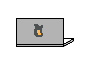
\includegraphics[scale=1.9]{Vectors/laptop_c.eps}\\
\vspace{0.4cm}
\begin{tabular}{c | c}
	Probability & Combination \\
	\midrule
	$p_1$ & \includegraphics[scale=0.06]{euro.jpg} $\quad$ \includegraphics[scale=0.06]{euro.jpg} $\quad$ \includegraphics[scale=0.06]{euro.jpg} \\
	$p_2$ & \includegraphics[scale=0.06]{euro.jpg} $\quad$ \includegraphics[scale=0.25]{euro_b.jpg} $\quad$ \includegraphics[scale=0.06]{euro.jpg} \\
	$p_3$ & \includegraphics[scale=0.06]{euro.jpg} $\quad$ \includegraphics[scale=0.06]{euro.jpg} $\quad$ \includegraphics[scale=0.26]{euro_b.jpg} \\
	. & . \\
	. & . \\
	. & . \\
	$p_8$ & \includegraphics[scale=0.26]{euro_b.jpg} $\quad$ \includegraphics[scale=0.26]{euro_b.jpg} $\quad$ \includegraphics[scale=0.26]{euro_b.jpg} \\
	
\end{tabular}
\end{minipage}%%%
\begin{minipage}[c]{0.49\textwidth}
\centering
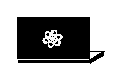
\includegraphics[scale=1.2]{Vectors/laptop_q.eps}\\
\vspace{0.5cm}
\begin{tabular}{c | c}
	Probability & Quantum state \\
	\midrule
	$p_1$ & \includegraphics[scale=0.03]{Vectors/black-atom-icon-free-vector.eps} $\quad$ \includegraphics[scale=0.03]{Vectors/black-atom-icon-free-vector.eps} $\quad$ \includegraphics[scale=0.03]{Vectors/black-atom-icon-free-vector.eps} \\
	$p_2$ & \includegraphics[scale=0.03]{Vectors/black-atom-icon-free-vector.eps} $\quad$ \includegraphics[scale=0.03]{Vectors/red-atom.eps} $\quad$ \includegraphics[scale=0.03]{Vectors/black-atom-icon-free-vector.eps} \\
	$p_3$ & \includegraphics[scale=0.03]{Vectors/black-atom-icon-free-vector.eps} $\quad$ \includegraphics[scale=0.03]{Vectors/black-atom-icon-free-vector.eps} $\quad$ \includegraphics[scale=0.03]{Vectors/red-atom.eps} \\
	. & . \\
	. & . \\
	. & . \\
	$p_8$ & \includegraphics[scale=0.03]{Vectors/red-atom.eps} $\quad$ \includegraphics[scale=0.03]{Vectors/red-atom.eps} $\quad$ \includegraphics[scale=0.03]{Vectors/red-atom.eps} \\
	
\end{tabular}
\end{minipage}

\end{frame}
}

{
\setbeamertemplate{frame footer}{\tiny{}}
\begin{frame}[fragile]{Three random bits vs. three qubits}

\begin{minipage}[c]{0.49\textwidth}
\centering
\includegraphics[scale=1.9]{Vectors/laptop_c.eps}\\
\vspace{0.4cm}
\begin{tabular}{c | c}
	Probability & Combination \\
	\midrule
	$p_1$ & 000 \\
	$p_2$ & 010 \\
	$p_3$ & 001 \\
	. & .\\
	. & . \\
	. & . \\
	$p_8$ & 111 \\
	
\end{tabular}
\end{minipage}%%%
\begin{minipage}[c]{0.49\textwidth}
\centering
\includegraphics[scale=1.2]{Vectors/laptop_q.eps}\\
\vspace{0.5cm}
\begin{tabular}{c | c}
	Probability & Quantum state \\
	\midrule
	$p_1$ & $\ket{000}$ \\
	$p_2$ & $\ket{010}$ \\
	$p_3$ & $\ket{001}$ \\
	. & . \\
	. & . \\
	. & . \\
	$p_8$ & $\ket{111}$ \\
	
\end{tabular}
\end{minipage}

\end{frame}
}

{
\setbeamertemplate{frame footer}{\tiny{}}
\begin{frame}[fragile]{Three random bits vs. three qubits}

\begin{minipage}[c]{0.39\textwidth}
\centering
\includegraphics[scale=1.9]{Vectors/laptop_c.eps}\\
\vspace{0.4cm}
\begin{tabular}{c | c}
	Prob. & Combination \\
	\midrule
	$p_1 = \frac{1}{8}$ & 000 \\
	$p_2= \frac{1}{8}$ & 010 \\
	$p_3= \frac{1}{8}$ & 001 \\
	. & .\\
	. & . \\
	. & . \\
	$p_8= \frac{1}{8}$ & 111 \\
	
\end{tabular}
\end{minipage}%%%
\begin{minipage}[c]{0.59\textwidth}
\centering
\includegraphics[scale=1.2]{Vectors/laptop_q.eps}\\
\vspace{0.5cm}
\begin{tabular}{c | c | c}
	Prob. & Amplitude & Quantum state \\
	\midrule
	$p_1 =\, \mid a_1\mid^2$ & $a_1$ & $\ket{000}$ \\
	$p_2 =\,\mid a_2\mid^2$ & $a_2$ & $\ket{010}$ \\
	$p_3 =\, \mid a_3\mid^2$ & $a_3$ & $\ket{001}$ \\
	. & .  & .\\
	. & . & .\\
	. & . & .\\
	$p_8 =\, \mid a_8\mid^2$ & $a_8$ & $\ket{111}$ \\
	
\end{tabular}
\end{minipage}
\end{frame}
}

{
\setbeamertemplate{frame footer}{\tiny{}}
\begin{frame}[fragile]{Three random bits vs. three qubits}

\begin{minipage}[c]{0.39\textwidth}
\centering
\includegraphics[scale=1.9]{Vectors/laptop_c.eps}\\
\vspace{0.4cm}
\begin{tabular}{c | c}
	Prob. & Combination \\
	\midrule
	$p_1 = \frac{1}{8}$ & 000 \\
	$p_2= \frac{1}{8}$ & 010 \\
	$p_3= \frac{1}{8}$ & 001 \\
	. & .\\
	. & . \\
	. & . \\
	$p_8= \frac{1}{8}$ & 111 \\
	
\end{tabular}
\end{minipage}%%%
\begin{minipage}[c]{0.59\textwidth}
\centering
\includegraphics[scale=1.2]{Vectors/laptop_q.eps}\\
\vspace{0.5cm}
\begin{tabular}{c | c | c}
	Prob. & Amplitude & Quantum state \\
	\midrule
	$p_1 = \mid\frac{1}{2\sqrt{2}}\mid^2 = \frac{1}{8}$ & $\frac{1}{2\sqrt{2}}$ & $\ket{000}$ \\
	$p_2 =\frac{1}{8}$ & $-\frac{1}{2\sqrt{2}}$ & $\ket{010}$ \\
	$p_3 = \frac{1}{8}$ & $-\frac{i}{2\sqrt{2}}$ & $\ket{001}$ \\
	. & .  & .\\
	. & . & .\\
	. & . & .\\
	$p_8 = \frac{1}{8}$ & $\frac{i}{2\sqrt{2}}$ & $\ket{111}$ \\
	
\end{tabular}
\end{minipage}\\
\vspace{0.5cm}
$\rightarrow$ In quantum mechanics amplitudes can be interferred with each other!\\
$\rightarrow$ This is impossible to do on a classical computer!
\end{frame}
}

{
\setbeamertemplate{frame footer}{\tiny{}}
\begin{frame}[fragile]{Three random bits vs. three qubits}

Applying an H gate to the first qubit leads to quantum interference such that:
\centering
\begin{figure}
\includegraphics[scale=1.2]{Vectors/laptop_q.eps}\\
\end{figure}
\vspace{0.5cm}
\begin{table}
\begin{tabular}{c | c | c}
	Prob. & Amplitude & Quantum state \\
	\midrule
	$p_1 = \,\mid a_1+a_5 \mid^2$ & $a_1+a_5$ & $\ket{000}$ \\
	$p_2 =\, \mid a_2+a_6 \mid^2$ & $a_2+a_6$ & $\ket{010}$ \\
	$p_3 = \,\mid a_3+a_7 \mid^2$ & $a_3+a_7$ & $\ket{001}$ \\
	$p_4 = \,\mid a_4+a_8 \mid^2$ & $a_4+a_8$ & $\ket{011}$ \\
	$p_5 = \,\mid a_1-a_5 \mid^2$ & $a_1-a_5$ & $\ket{100}$ \\
	$p_6 = \,\mid a_2-a_6 \mid^2$ & $a_2-a_6$ & $\ket{110}$ \\
	$p_7 = \,\mid a_3-a_7 \mid^2$ & $a_3-a_7$ & $\ket{101}$ \\
	$p_8 = \,\mid a_4-a_8 \mid^2$ & $a_4-a_8$ & $\ket{111}$ \\
	
\end{tabular}
\end{table}

\end{frame}
}

{
\setbeamertemplate{frame footer}{\tiny{}}
\begin{frame}[fragile]{Three random bits vs. three qubits}

For example, substituting the values for $a_1=\frac{1}{2\sqrt{2}}$ and $a_5=\frac{1}{2\sqrt{2}}$ yields:
\centering
\begin{figure}
\includegraphics[scale=1.2]{Vectors/laptop_q.eps}\\
\end{figure}
\vspace{0.5cm}
\begin{table}
\begin{tabular}{c | c | c}
	Prob. & Amplitude & Quantum state \\
	\midrule
	$p_1 = \,\mid a_1+a_5 \mid^2$ & $\frac{1}{\sqrt{2}}(\frac{1}{2\sqrt{2}}+\frac{1}{2\sqrt{2}})$ & $\ket{000}$ \\
	$p_2 =\, \mid a_2+a_6 \mid^2$ & $a_2+a_6$ & $\ket{010}$ \\
	$p_3 = \,\mid a_3+a_7 \mid^2$ & $a_3+a_7$ & $\ket{001}$ \\
	$p_4 = \,\mid a_4+a_8 \mid^2$ & $a_4+a_8$ & $\ket{011}$ \\
	$p_5 = \,\mid a_1-a_5 \mid^2$ & $\frac{1}{\sqrt{2}}(\frac{1}{2\sqrt{2}}-\frac{1}{2\sqrt{2}})$ & $\ket{100}$ \\
	$p_6 = \,\mid a_2-a_6 \mid^2$ & $a_2-a_6$ & $\ket{110}$ \\
	$p_7 = \,\mid a_3-a_7 \mid^2$ & $a_3-a_7$ & $\ket{101}$ \\
	$p_8 = \,\mid a_4-a_8 \mid^2$ & $a_4-a_8$ & $\ket{111}$ \\
	
\end{tabular}
\end{table}

\end{frame}
}

{
\setbeamertemplate{frame footer}{\tiny{}}
\begin{frame}[fragile]{Three random bits vs. three qubits}

For example, substituting the values for $a_1 = \frac{1}{2\sqrt{2}}$ and $a_5 = \frac{1}{2\sqrt{2}}$ yields:
\centering
\begin{figure}
\includegraphics[scale=1.2]{Vectors/laptop_q.eps}\\
\end{figure}
\vspace{0.5cm}
\begin{table}
\begin{tabular}{c | c | c c}
	Prob. & Amplitude & Quantum state &  \\
	\midrule
	$p_1 = \,\mid \frac{1}{2} \mid^2 = \frac{1}{4}$ & $\frac{1}{2}$ & $\ket{000}$ & $\rightarrow$ constructive interference \\
	$p_2 =\, \mid a_2+a_6 \mid^2$ & $a_2+a_6$ & $\ket{010}$ & " \\
	$p_3 = \,\mid a_3+a_7 \mid^2$ & $a_3+a_7$ & $\ket{001}$ & "\\
	$p_4 = \,\mid a_4+a_8 \mid^2$ & $a_4+a_8$ & $\ket{011}$ & "\\
	$p_5 = \,\mid 0 \mid^2 = 0$ & $0$ & $\ket{100}$ & $\rightarrow$ destructive interference \\
	$p_6 = \,\mid a_2-a_6 \mid^2$ & $a_2-a_6$ & $\ket{110}$ & "\\
	$p_7 = \,\mid a_3-a_7 \mid^2$ & $a_3-a_7$ & $\ket{101}$ & "\\
	$p_8 = \,\mid a_4-a_8 \mid^2$ & $a_4-a_8$ & $\ket{111}$ & "\\
	
\end{tabular}
\end{table}

\end{frame}
}

{
\setbeamertemplate{frame footer}{\tiny{\textsuperscript{1}}}
\begin{frame}[fragile]{Calculating distances with interference}
\hspace{-0.7cm}
\begin{minipage}[c]{0.29\textwidth}
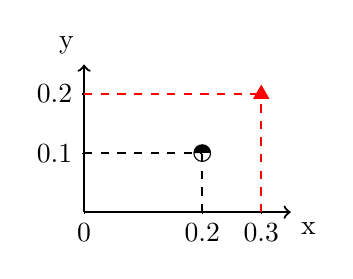
\begin{tikzpicture}[scale=0.75]
%define the axes
\draw[thick,->] (0,0) -- (3.5,0) node[anchor=north west] {x};
\draw[thick,->] (0,0) -- (0,2.5) node[anchor=south east] {y};
\draw (0 cm,1pt) -- (0 cm,-1pt) node[anchor=north] {$0$};
%\draw (1 cm,1pt) -- (1 cm,-1pt) node[anchor=north] {$0.1$};
\draw (2 cm,1pt) -- (2 cm,-1pt) node[anchor=north] {$0.2$};
\draw (3 cm,1pt) -- (3 cm,-1pt) node[anchor=north] {$0.3$};
%\draw (4 cm,1pt) -- (4 cm,-1pt) node[anchor=north] {$0.4$};
%\draw (5 cm,1pt) -- (5 cm,-1pt) node[anchor=north] {$0.5$};
\draw (1pt,1 cm) -- (-1pt,1 cm) node[anchor=east] {$0.1$};
\draw (1pt,2 cm) -- (-1pt,2 cm) node[anchor=east] {$0.2$};
%\draw (1pt,3 cm) -- (-1pt,3 cm) node[anchor=east] {$0.3$};
%\draw (1pt,4 cm) -- (-1pt,4 cm) node[anchor=east] {$0.4$};
%\draw (1pt,5 cm) -- (-1pt,5 cm) node[anchor=east] {$0.5$};
%draw the dotted lines to the first point
\draw[black,thick,dashed] (2,0) -- (2, 1);
\draw[black,thick,dashed] (0,1) -- (2, 1);
%draw the dotted lines to the second point
\draw[red,thick,dashed] (3,0) -- (3, 2);
\draw[red,thick,dashed] (0,2) -- (3, 2);
%draw the two point markerss
\node[mark size=3pt,color=red] at (3,2) {\pgfuseplotmark{triangle*}};
\node[mark size=3pt,color=black] at (2,1) {\pgfuseplotmark{halfcircle*}};
\end{tikzpicture}
\end{minipage}%%%
\hspace{0.55cm}
\begin{minipage}[c]{0.69\textwidth}
\centering
\includegraphics[scale=1.2]{Vectors/laptop_q.eps}\\
\vspace{0.5cm}
\flushright
\begin{tabular}{c | c | c c}
	Prob. & Amplitude & Quantum state  \\
	\midrule
	$p_1 = 0.22 $ & $\frac{0.2}{\sqrt{0.18}}$ & $\ket{000}$\\
	$p_2 = 0.055$ & $\frac{0.1}{\sqrt{0.18}}$ & $\ket{010}$  \\
	$p_3= 0$ & $0$ & $\ket{001}$ \\
	$p_4 = 0$ & $0$ & $\ket{011}$ \\
	$p_5 = 0.5$ & $\frac{0.3}{\sqrt{0.18}}$ & $\ket{100}$  \\
	$p_6= 0.22$ & $\frac{0.2}{\sqrt{0.18}}$ & $\ket{110}$ \\
	$p_7 = 0$ & $0$ & $\ket{101}$ \\
	$p_8 = 0$ & $0$ & $\ket{111}$\\
	
\end{tabular}
\end{minipage}

\end{frame}
}

{
\setbeamertemplate{frame footer}{\tiny{\textsuperscript{1}}}
\begin{frame}[fragile]{Calculating distances with interference}
\hspace{-0.7cm}
\begin{minipage}[c]{0.29\textwidth}
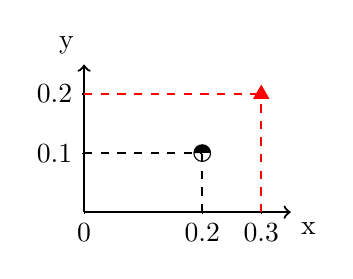
\begin{tikzpicture}[scale=0.75]
%define the axes
\draw[thick,->] (0,0) -- (3.5,0) node[anchor=north west] {x};
\draw[thick,->] (0,0) -- (0,2.5) node[anchor=south east] {y};
\draw (0 cm,1pt) -- (0 cm,-1pt) node[anchor=north] {$0$};
%\draw (1 cm,1pt) -- (1 cm,-1pt) node[anchor=north] {$0.1$};
\draw (2 cm,1pt) -- (2 cm,-1pt) node[anchor=north] {$0.2$};
\draw (3 cm,1pt) -- (3 cm,-1pt) node[anchor=north] {$0.3$};
%\draw (4 cm,1pt) -- (4 cm,-1pt) node[anchor=north] {$0.4$};
%\draw (5 cm,1pt) -- (5 cm,-1pt) node[anchor=north] {$0.5$};
\draw (1pt,1 cm) -- (-1pt,1 cm) node[anchor=east] {$0.1$};
\draw (1pt,2 cm) -- (-1pt,2 cm) node[anchor=east] {$0.2$};
%\draw (1pt,3 cm) -- (-1pt,3 cm) node[anchor=east] {$0.3$};
%\draw (1pt,4 cm) -- (-1pt,4 cm) node[anchor=east] {$0.4$};
%\draw (1pt,5 cm) -- (-1pt,5 cm) node[anchor=east] {$0.5$};
%draw the dotted lines to the first point
\draw[black,thick,dashed] (2,0) -- (2, 1);
\draw[black,thick,dashed] (0,1) -- (2, 1);
%draw the dotted lines to the second point
\draw[red,thick,dashed] (3,0) -- (3, 2);
\draw[red,thick,dashed] (0,2) -- (3, 2);
%draw the two point markerss
\node[mark size=3pt,color=red] at (3,2) {\pgfuseplotmark{triangle*}};
\node[mark size=3pt,color=black] at (2,1) {\pgfuseplotmark{halfcircle*}};
\end{tikzpicture}
\end{minipage}%%%
\hspace{0.55cm}
\begin{minipage}[c]{0.69\textwidth}
\centering
\includegraphics[scale=1.2]{Vectors/laptop_q.eps}\\
\vspace{0.5cm}
\flushright
\begin{tabular}{c | c | c c}
	Prob. & Amplitude & Quantum state  \\
	\midrule
	$p_1 =\, \frac{(0.2+0.3)^2}{0.18}$ & $\frac{0.2+0.3}{\sqrt{0.18}}$ & $\ket{000}$\\
	$p_2 =\, \frac{(0.1+0.2)^2}{0.18}$ & $\frac{0.1+0.2}{\sqrt{0.18}}$ & $\ket{010}$  \\
	$p_3 = 0$ & $0$ & $\ket{001}$ \\
	$p_4 = 0$ & $0$ & $\ket{011}$ \\
	$p_5 = \,\frac{(0.2-0.3)^2}{0.18}$ & $\frac{0.2-0.3}{\sqrt{0.18}}$ & $\ket{100}$  \\
	$p_6 = \, \frac{(0.1-0.2)^2}{0.18}$ & $\frac{0.1-0.2}{\sqrt{0.18}}$ & $\ket{110}$ \\
	$p_7 = 0$ & $0$ &  $\ket{101}$ \\
	$p_8 = 0$ & $0$ &  $\ket{111}$\\
	
\end{tabular}
\end{minipage}
\end{frame}
}

{
\setbeamertemplate{frame footer}{\tiny{\textsuperscript{1}Nielsen, M. A., \& Chuang, I. L. (2010). Quantum computation and quantum information. Cambridge University Press.\newline \textsuperscript{2}Jat, R. N., \& Ruhela, D. S. (2011). Comparative study of complexity of algorithms for iterative solution of non-linear equations. Journal of International Academy Of Physical Sciences, 15(4).}}
\begin{frame}{Controlled U gate}

\begin{minipage}[t]{.4\textwidth}
	%\vspace{-20mm}
	\includegraphics[height=0.5\textwidth]{controlledU.png}
       \captionsetup{justification=raggedright, singlelinecheck=false}
       \captionof{figure}{\footnotesize{Controlled U-gate} }
\end{minipage}%%%%%
\begin{minipage}[t]{.6\textwidth}
%\vspace{-20mm}
\includegraphics[width=1\textwidth]{controlledUdecomposition.png}
       \captionsetup{justification=raggedright, singlelinecheck=false}
       \captionof{figure}{\footnotesize{Decomposition of a controlled U-gate\textsuperscript{1}} }
\end{minipage}

Choose A,B,C and $\alpha$ s.t.
\begin{equation}
e^{i\alpha}*A*X*B*X*C = U \quad and \quad A*B*C = \mathds{1}
\end{equation}
Need to solve the following equation\textsuperscript{1}
\begin{equation}
U = \begin{pmatrix}
 e^{i(\alpha-\frac{\beta}{2}-\frac{\delta}{2})}\cos{\frac{\gamma}{2}} & -e^{i(\alpha-\frac{\beta}{2}+\frac{\delta}{2})}\sin{\frac{\gamma}{2}} \\ 
e^{i(\alpha+\frac{\beta}{2}-\frac{\delta}{2})}\sin{\frac{\gamma}{2}} & e^{i(\alpha+\frac{\beta}{2}+\frac{\delta}{2})}\cos{\frac{\gamma}{2}}
 \end{pmatrix}
\end{equation}

%calculating a root of a function f(x) with n-digit precision, provided that a good initial approximation is known, is O((\log n) F(n)) where F(n) is the cost of calculating f(x)/f'(x)\, with n-digit precision.

	%\metroset{block=fill}
	%\begin{alertblock}{Overall algorithmic complexity}
	%$\mathcal{O}(\frac{1}{p_{acc}})+\textcolor{red}{\mathcal{O}(k)}$ where $k$ is number of root finding iterations\textsuperscript{2}
	%\end{alertblock}
\end{frame}

}{
\setbeamertemplate{frame footer}{\tiny{\textsuperscript{1}Dawson, C. M., \& Nielsen, M. A. (2005). The Solovay-Kitaev algorithm. arXiv preprint quant-ph/0505030.}}
\begin{frame}{Problems with universal gate sets}

In our case we need to find A, B, C and $\alpha$ for $_0^1CR_y(\frac{\pi}{4})$:

Using a root finding algorithm for non-linear equations we find:

\begin{equation}
\alpha =  \pi; \quad 
\beta = 2\pi;\quad 
\delta = \frac{7}{8}\pi;\quad 
\gamma = 0
\end{equation}
Then,
\begin{align}
A \quad= \quad R_z(\beta)R_y(\frac{\gamma}{2})\quad =& \quad R_z(2\pi) \quad = \quad \textcolor{emerald}{\mathds{1}} \\
B\quad =\quad R_y(-\frac{\gamma}{2})R_z(-\frac{\delta+\beta}{2})\quad =& \quad R_z(-\frac{23}{16}\pi) \quad= \quad \textcolor{red}{???}  \\
C \quad=\quad R_z(\frac{\delta-\beta}{2})\quad =& \quad R_z(-\frac{9}{16}\pi) \quad= \quad \textcolor{red}{???} \\
\begin{pmatrix} 1&0\cr0&e^{i\alpha} \end{pmatrix}\quad=& \quad \begin{pmatrix} 1&0\cr0&e^{i\pi} \end{pmatrix}\quad= \quad \textcolor{emerald}{Z}
\end{align}

\end{frame}
}

{
\setbeamertemplate{frame footer}{\tiny{\textsuperscript{1}Dawson, C. M., \& Nielsen, M. A. (2005). The Solovay-Kitaev algorithm. arXiv preprint quant-ph/0505030.}}
\begin{frame}{The Solovay-Kitaev theorem}

\begin{align}
B\quad =&\quad R_z(-\frac{23}{16}\pi) \quad= \quad \textcolor{red}{???}  \\
C \quad=&\quad R_z(-\frac{9}{16}\pi) \quad= \quad \textcolor{red}{???}
\end{align}

The Solovay-Kitaev theorem guarantees that given a set of single-qubit quantum gates which generates a dense subset of $SU(2)$, then that set is guaranteed to fill $SU(2)$ quickly.\textsuperscript{1}
 
$\rightarrow$ \textcolor{emerald}{\textbf{Hence, given any universal gate set it is possible to obtain good approximations to any desired gate.}}

$\rightarrow$ \textcolor{red}{\textbf{But needs to be computed classically!}}

\end{frame}
}

{
\setbeamertemplate{frame footer}{\tiny{\textsuperscript{1}Booth Jr, J. (2012). Quantum compiler optimizations. arXiv preprint arXiv:1206.3348.}}
\begin{frame}{The Solovay-Kitaev algorithm}

Fowler distance\textsuperscript{1}:
\begin{equation}
dist(U,U_{approx}) = \sqrt{\frac{2-\mid tr(U\cdot U_{approx}^\dagger)\mid}{2}}
\end{equation}

\begin{figure}
    \begin{tikzpicture}[scale=0.8]
\begin{axis}[xlabel={Gate count},ylabel={Fowler distance [$d(U,U_{approx})$]}]

% Graph column 2 versus column 0
\addplot table[x index=1,y index=0,col sep=comma] {datax.dat};
\addlegendentry{$R_z(-\frac{9}{16}\pi)$}% y index+1 since humans count from 1

% Graph column 1 versus column 0    
\addplot table[x index=5,y index=4,col sep=comma] {datax.dat};
\addlegendentry{$R_z(-\frac{23}{16}\pi)$}

\end{axis}
\end{tikzpicture}
  \end{figure}

\end{frame}
}

{
\setbeamertemplate{frame footer}{}
\begin{frame}{The Solovay-Kitaev algorithm}

\begin{minipage}[c]{.8\textwidth}
	%\vspace{-20mm}
	\includegraphics[height=0.8\textwidth]{fowlerdistance.png}
       \captionsetup{justification=raggedright, singlelinecheck=false}
       \captionof{figure}{\footnotesize{Various Fowler distances visualized on Bloch sphere} }
\end{minipage}%%%%%
\begin{minipage}[c]{.2\textwidth}
\scriptsize
\begin{equation}
\textcolor{cyan}{d = 0.22739}
\end{equation}
\begin{equation}
\textcolor{emerald}{d = 0.15165}
\end{equation}
\begin{equation}
\textcolor{blue}{d = 0.10722}
\end{equation}
\begin{equation}
\textcolor{darkyellow}{d = 0.02086}
\end{equation}
\begin{equation}
\textcolor{red}{d = 0.00156}
\end{equation}

\end{minipage}

\end{frame}
}

{
\setbeamertemplate{frame footer}{}
\begin{frame}{The Solovay-Kitaev algorithm}

IBM's quantum computer needs \textbf{130ns for single-qubit gates} and \textbf{500ns for CNOT gates.}

IBM qubit decoherence times:

\SI{49.5}{\micro\second} $\leq T_1 \leq$ \SI{85.3}{\micro\second} "amplitude damping"\\
\SI{56.0}{\micro\second} $\leq T_2 \leq$ \SI{139.7}{\micro\second} "phase damping"
\vspace{6mm}


\begin{table}
    \begin{tabular}{c| c |c |c }
      \toprule
      Approx. Gate & Distance & Gate count & Execution time\\
      \midrule
      $R_z(-\frac{23}{16}\pi)$ & 0.15165 & 25 & \textcolor{emerald}{$\sim$\SI{3}{\micro\second}}\\
       & 0.10722 & 109 & \textcolor{emerald}{$\sim$\SI{14}{\micro\second}}\\
       & 0.02086 & 2997 & \textcolor{red}{$\sim$\SI{390}{\micro\second}}\\
       & 0.01494 & 14721 & \textcolor{red}{$\sim$\SI{1914}{\micro\second}}\\
       & 0.003327 & 74009 & \textcolor{red}{$\sim$\SI{9621}{\micro\second}}\\
       & 0.001578 & 370813 & \textcolor{red}{$\sim$\SI{48206}{\micro\second}}\\
      \bottomrule
    \end{tabular}
    \caption{SK algorithm results}
  \end{table}
 

\end{frame}
}

{
\setbeamertemplate{frame footer}{\tiny{\textsuperscript{1}}}
\begin{frame}[fragile]{Encoding classical data into qubits}

%There are two different ways for encoding classical data into quantum states: 

\begin{alertblock}{1. Data encoded into qubits}
%speed-up not very clear since the \# of qubits increases linearly with the \# of classical bits
k-dimensional probability vector requires $4k$ classical bits which are encoded one-to-one into $4k$ qubits, e.g.\\
\vspace{2mm}
$\begin{pmatrix}
 \textcolor{blue}{0.6} \\ 
 \textcolor{emerald}{0.4}
 \end{pmatrix}*10 \rightarrow \begin{pmatrix}
 \textcolor{blue}{6} \\ 
 \textcolor{emerald}{4}
 \end{pmatrix} \rightarrow \begin{pmatrix}
 \textcolor{blue}{0110} \\ 
 \textcolor{emerald}{0100}
 \end{pmatrix} \rightarrow n=\textcolor{blue}{0110}\textcolor{emerald}{0100} \rightarrow \ket{n} = \ket{\textcolor{blue}{0110}\textcolor{emerald}{0100}}$\\
%\textbf{Only slight speed up possible}
\end{alertblock}
\vspace{1cm}
Schuld, Sinayskiy, and Petruccione (2014) developed a \textbf{qubit-based} quantum kNN algorithm. $\rightarrow$ requires a lot of qubits\\
\vspace{0.5cm}
My thesis research stressed the need for an alternative...


\end{frame}
}

\end{document}
